%!TEX program = xelatex
% Original author content: CC-BY-4.0. Third-party rights are retained.
\documentclass[11pt,a4paper]{article}
\usepackage[margin=2.4cm]{geometry}
\usepackage{fontspec}
\setmainfont{lmroman10-regular.otf}[BoldFont=lmroman10-bold.otf,ItalicFont=lmroman10-italic.otf,BoldItalicFont=lmroman10-bolditalic.otf]
\setsansfont{lmsans10-regular.otf}[BoldFont=lmsans10-bold.otf,ItalicFont=lmsans10-oblique.otf,BoldItalicFont=lmsans10-boldoblique.otf]
\setmonofont{lmmono10-regular.otf}[ItalicFont=lmmono10-italic.otf]
\usepackage{amsmath,amssymb,booktabs,graphicx,float,tabularx,array,multirow,makecell,threeparttable}
\usepackage{caption,subfigure,setspace,fancyhdr,chngcntr}
\usepackage[numbers,sort&compress]{natbib}
\usepackage[hidelinks,unicode]{hyperref}
\hypersetup{pdftitle={Stock Volatility Forecasting with MIDAS EPU Correction},pdfauthor={Boursin Nickel},pdfsubject={English research edition; version 0.5-review; original content CC BY 4.0}}
\setstretch{1.2}\setlength{\headheight}{15pt}
\pagestyle{fancy}\fancyhf{}\fancyhead[C]{\small Volatility Forecasting with MIDAS EPU Correction}\fancyfoot[C]{\thepage}
\counterwithin{table}{section}\counterwithin{figure}{section}\counterwithin{equation}{section}
\setlength{\emergencystretch}{3em}
\begin{document}
\begin{titlepage}\centering\vspace*{2.6cm}
{\LARGE\bfseries Stock Volatility Forecasting\\[0.5em]with MIDAS EPU Correction\par}
\vspace{1cm}{\Large Stable Estimation, Residual Ablation,\\and Retrospective Reanalysis\par}
\vspace{2cm}{\Large Boursin Nickel\par}
\vspace{0.8cm}{\large English research edition\par}
\vfill
Version 0.5-review\par
2026-10-31\par
\vspace{1cm}
\begin{minipage}{0.87\textwidth}\centering
This edition reports the same revised experiments as the Chinese research manuscript. Historical evidence is retained separately. The analysis is exploratory and retrospective; it does not establish real-time forecasting validity.
\end{minipage}
\end{titlepage}
\pagenumbering{Roman}
\section*{Edition and licensing}
\thispagestyle{plain}
Copyright \copyright\ 2026 Boursin Nickel.

The author's licensable paper text, narrative documentation, and original figures and tables are licensed under \href{https://creativecommons.org/licenses/by/4.0/}{Creative Commons Attribution 4.0 International (CC BY 4.0)}. Give appropriate credit, link the license, and indicate modifications without implying endorsement. The complete terms are provided in the accompanying \texttt{LICENSE-CONTENT.txt}.

The author's licensable project code, executable examples, and runtime configurations are licensed under the Apache License, Version 2.0; see the project-root \texttt{LICENSE}. Third-party citations, adapted code, and embedded fonts retain their respective rights and conditions; see \texttt{THIRD\_PARTY\_NOTICES.md}. Neither project license grants rights to obtain, use, or redistribute underlying market or economic policy uncertainty data.

This is an English research edition of the Chinese public revision, reorganized for readability rather than translated sentence by sentence. It preserves the experimental definitions, results, historical controls, and limitations. It is not a separate experiment or an independently validated replication. The date identifies this local revision, not a journal publication or a public repository release.

Code citation metadata is supplied in \texttt{CITATION.cff}; edition-specific paper citations and compilation instructions are in \texttt{paper/README.md}. No repository URL, DOI, or publication venue is asserted.
\clearpage
\section*{Abstract}
\addcontentsline{toc}{section}{Abstract}
This study examines whether monthly economic policy uncertainty (EPU) information improves daily stock-index volatility-proxy forecasts after accounting for predictable errors in a market-only machine-learning model. The target is the logarithm of the next trading day's squared return plus a small offset. Comparisons include HAR, Student-$t$ GARCH(1,1), XGB-Market, a residual-only autoregressive correction (XGB-AR), and a mixed-data sampling (MIDAS) dynamic error correction (DEC) model.

A retrospective audit motivates three revisions: bounded multistart estimation with an analytic profiled gradient, removal of a confirmed SSE50 holiday record before feature construction, and a residual-only ablation. Specifications are selected using validation MSE, not test loss. For CSI300, revised DEC has log-MSE 5.112644 versus 5.099716 for XGB-Market, but QLIKE 3.536964 versus 4.951636. Relative to XGB-AR, DEC reduces QLIKE and increases MSE in all three markets; its MAE advantage is confined to the two Chinese markets. Nasdaq's selected specification changes from a 12-month Beta weighting scheme to a 12-month exponential Almon scheme. Relative to archived DEC, its MSE improves while QLIKE deteriorates.

Five models are evaluated under 30 rolling-residual interval settings. On 1859 common dates, 90\% intervals with a calibration window of 250 give DEC an interval score of 10.1995, compared with 9.6973 for HAR, 9.8534 for XGB-Market, and 9.8793 for XGB-AR. DEC therefore does not improve interval quality against these benchmarks. These intervals concern an observed proxy, not latent conditional variance.

All 6888 archived XGBoost predictions can be matched using a documented sampling-compatible build. The original DEC numerical environment remains unidentified. Revised DEC predictions differ by less than $10^{-7}$ across the two examined numerical-library stacks, but numerical stability is not proof of a global optimum. Missing real-time EPU vintages, prior exposure to historical results, model selection, and dependence limit inferential claims. The contribution is a reproducible correction and comparison framework with loss-dependent findings, not evidence of universal forecasting superiority or a causal EPU effect.

\medskip
\noindent\textbf{Keywords:} volatility proxy; economic policy uncertainty; MIDAS; XGBoost; dynamic error correction; numerical reproducibility; prediction intervals.
\clearpage

\tableofcontents\clearpage
\pagenumbering{arabic}
\section{Introduction}
\label{sec:introduction}
Volatility forecasts are sensitive to both the information set and the quantity being predicted. Persistent volatility, nonlinear responses to market conditions, and low-frequency macroeconomic indicators motivate models that combine daily market information with monthly economic policy uncertainty (EPU). Yet an apparent improvement can also reflect predictable residual dynamics, a different loss function, data preparation errors, or numerical optimization behavior. A useful comparison must distinguish these mechanisms rather than treat every lower reported loss as evidence of a better economic model.

This study uses a market-only XGBoost predictor as a first stage and models its realized forecast errors in a second stage. A MIDAS-weighted monthly EPU signal enters alongside a lagged error. A residual-only correction supplies the relevant ablation: it asks whether the EPU component adds predictive information beyond error persistence. The target is a daily squared-return proxy, not high-frequency realized variance. This distinction matters for interpretation and for comparisons with the realized-volatility literature.

ARCH and GARCH model conditional heteroskedasticity directly \citep{Engle1982,Bollerslev1986}. Research on realized volatility uses intraday information to construct more informative ex post measures \citep{AndersenBollerslevDieboldLabys2003}; the HAR framework captures persistence across horizons \citep{Corsi2009}. Here, HAR-style daily, weekly, and monthly features are constructed from daily squared returns, so results should not be described as tests of a full intraday realized-volatility implementation. Extensions such as realized kernels and jump-robust measures are relevant alternatives but are not implemented in this experiment.

News-based EPU indices measure the prevalence of policy-related economic uncertainty in specified sources \citep{BakerBloomDavis2016,DavisLiuSheng2019}. Prior work links EPU to stock-market volatility \citep{LiuZhang2015}, while MIDAS and GARCH-MIDAS provide established methods for combining sampling frequencies \citep{GhyselsSinkoValkanov2007,EngleGhyselsSohn2013}. The present second stage is not GARCH-MIDAS: it corrects a log-target point forecast using a weighted EPU signal and an observed lagged forecast error. EPU is not treated as an exogenous policy shock, and a nonzero fitted coefficient does not identify a causal effect.

XGBoost provides a regularized boosted-tree implementation \citep{ChenGuestrin2016}. Evidence on machine learning in empirical asset pricing \citep{GuKellyXiu2020} motivates nonlinear modeling, but does not by itself establish an advantage for this target or data set. The market-only baseline and its residual-only correction are therefore essential comparisons. Standard HAR and GARCH remain informative, although the benchmark set is not exhaustive.

Evaluation also depends on the forecast target and loss. Proxy-robust loss rankings require conditions on the proxy \citep{Patton2011}; those conditions cannot simply be assumed after nonlinear transformations and numerical floors. Forecast-comparison tests \citep{DieboldMariano1995,ClarkWest2007} are not automatically valid for every estimated, selected, or nested model. Coverage diagnostics \citep{Christoffersen1998} and interval scores \citep{GneitingRaftery2007} reveal properties that point losses omit. Although the interval construction uses conformal-style order statistics, it is not an implementation of EnbPI and does not inherit that method's guarantees \citep{Vovk2005,ShaferVovk2008,Lei2018,XuXie2021}.

The study has three practical aims. First, it reconciles archived data, configurations, and numerical results. Second, it reassesses the incremental EPU component using a stable solver, a residual ablation, and multiple losses. Third, it evaluates interval behavior and compares markets while preserving the distinction between current and historical results. The resulting contribution is an auditable empirical reanalysis, not a claim to invent MIDAS, boosting, error correction, or conformal prediction. The literature comparison is selective rather than a systematic review, and no priority claim is made.

The design is retrospective. Historical results were already known before the current revision, and the additional markets are not untouched external validation samples. Data-snooping concerns therefore remain even when the revised estimation and validation rules are fixed before inspecting the newly computed test results \citep{LoMacKinlay1990,HarveyLiuZhu2016}. Confirmatory evidence would require a locked design and new observations with documented real-time information availability.

\begin{figure}[htbp]
\centering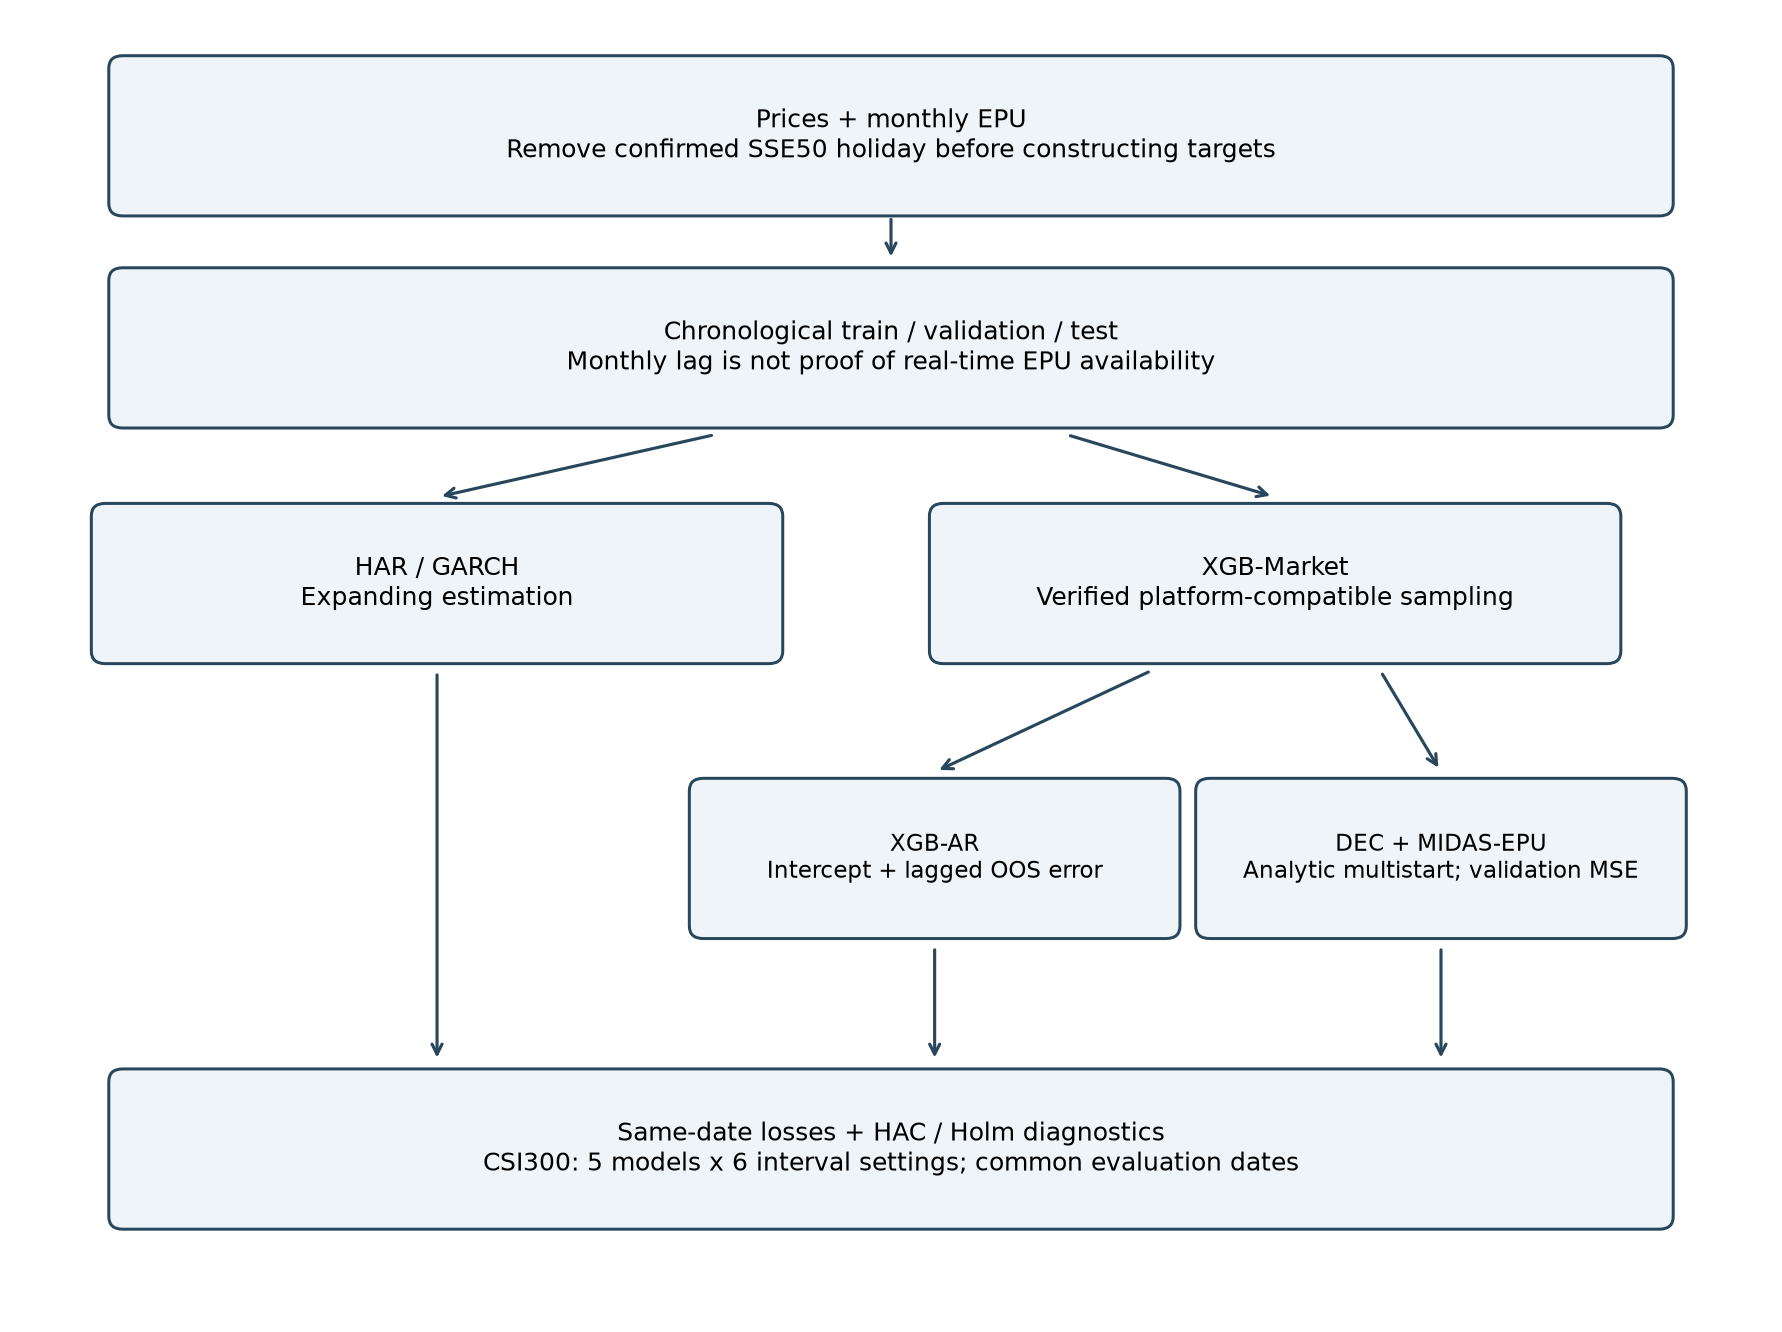
\includegraphics[width=\textwidth]{../../results/revised/method_flow.png}
\caption{Current workflow. Numerical checks, residual ablation, and common-date interval evaluation are separated from historical reproduction.}
\label{fig:f}
\end{figure}

Section~\ref{sec:methods} defines the data, models, estimation, and evaluation rules. Sections~\ref{sec:point} and~\ref{sec:intervals} report CSI300 point and interval results. Section~\ref{sec:robustness} examines SSE50 and Nasdaq. The conclusion and appendices state the reproducibility boundaries and historical controls.
\clearpage

\section{Data and methods}
\label{sec:methods}
\subsection{Target and interpretation}
Let $C_t$ denote a daily closing price and define
\begin{equation}
r_t=\log(C_t/C_{t-1}),\qquad RV_t=r_t^2,\qquad
 y_{t+1}=\log(RV_{t+1}+\varepsilon),\quad\varepsilon=10^{-8}.
\end{equation}
The notation $RV_t$ follows the project code; it is a daily squared return, not a sum of intraday squared returns. Its conditional expectation is a conditional second moment, equal to conditional variance only when the conditional mean return is zero. Forecasts are mapped back by
\begin{equation}
\widehat{RV}_{t+1|t}=\max\{\exp(\widehat y_{t+1|t})-\varepsilon,10^{-12}\}.
\end{equation}
A model minimizing squared error in the log target estimates a different functional from one modeling conditional variance directly. By Jensen's inequality, exponentiating a conditional mean of the log target does not generally recover the conditional mean of the untransformed target. Consequently, disagreement between log-MSE and QLIKE rankings need not imply an implementation error.

\subsection{Inputs, sample construction, and data audit}
The study uses daily CSI300, SSE50, and Nasdaq market records, monthly Chinese EPU for the Chinese indices, and monthly US EPU for Nasdaq. The Chinese series is the mainland-newspaper measure cited in \citet{DavisLiuSheng2019}, rather than an interchangeable substitute for every published Chinese EPU series. Its newspaper sources include the People's Daily and Guangming Daily. The original EPU download versions, release timestamps, and revision histories are not fully archived. Lagging monthly observations reduces contemporaneous overlap but cannot establish a genuine real-time information set.

The CSI300 descriptive sample spans January 2010 to March 2026. Its 3942 prices yield 3941 returns. An archived descriptive output instead contained 3942 returns. Inserting an additional zero between the observations dated 2018-06-15 and 2018-06-19 reproduces 24 historical statistical fingerprints; the historical operation that created that extra observation remains unknown. This insertion is a forensic diagnostic only and is not used for current descriptive statistics or model estimation. The reconciled CSI300 model matrix has 3919 rows without that added zero.

For SSE50, a confirmed holiday record dated 2018-06-18 had zero volume and an unchanged close. Removing that row only after target construction would leave an artificial $\log(10^{-8})$ target on the preceding retained observation. The current pipeline removes the confirmed holiday before constructing returns, features, and targets, consistent with the Shanghai Stock Exchange's 2018 holiday schedule announced on 2017-12-22. Zero volume alone is not used to classify all other dates as holidays. This correction is not a complete audit of every market's calendar or upstream data source.

\begin{table}[htbp]\centering
\caption{Current chronological sample definitions. Dates identify forecast origins.}
\begin{tabular}{lrrrr}\toprule
Market & Prepared & Initial train & Validation & Test\\\midrule
CSI300 & 3919 & 1500 & 500 & 1919\\
SSE50, corrected & 3919 & 1500 & 500 & 1919\\
Nasdaq & 4054 & 2000 & 500 & 1554\\\bottomrule
\end{tabular}
\begin{flushleft}\small CSI300 and corrected SSE50 test origins: 2018-05-03 to 2026-03-30. Nasdaq: 2020-01-23 to 2026-03-30. Historical SSE50 had 3915 prepared rows and 1915 test rows. These counts describe the recorded inputs, not a requirement for arbitrary new data.\end{flushleft}
\label{tab:samples}
\end{table}

The original archived model matrices were reconciled by dates, features, 24 EPU lags, targets, and sample flags. Matching an archive establishes provenance consistency, not that all upstream observations are error-free. Current descriptive statistics and diagnostics use the corrected 3941-return series (Tables~\ref{tab:desc_return_short} and~\ref{tab:diagnostic_tests_short}). The sample exhibits heavy tails and dependence in squared returns, motivating volatility models without establishing any particular specification as correct.

\begin{table}[htbp]\centering
\caption{CSI300 daily log-return descriptive statistics.}
\label{tab:desc_return_short}
\begin{tabular}{lr}\toprule Statistic & Value\\\midrule
Observations & 3941\\
Mean & $5.8396\times10^{-5}$\\
Standard deviation & 0.013639\\
Minimum & $-0.091544$\\
Maximum & 0.081420\\
Skewness & $-0.576130$\\
Excess kurtosis & 5.460548\\\bottomrule
\end{tabular}
\end{table}
\begin{table}[htbp]\centering
\caption{Distributional and dependence diagnostics for CSI300 returns.}
\label{tab:diagnostic_tests_short}
\begin{tabular}{lrr}\toprule Test & Statistic & $p$-value\\\midrule
Jarque--Bera & 5099.01 & $<0.0001$\\
Ljung--Box, returns, 10 lags & 32.75 & 0.0003\\
Ljung--Box, returns, 20 lags & 64.45 & $1.43\times10^{-6}$\\
Ljung--Box, squared returns, 10 lags & 1051.71 & $1.35\times10^{-219}$\\
Ljung--Box, squared returns, 20 lags & 1526.13 & $9.87\times10^{-312}$\\
ARCH LM, 10 lags & 452.36 & $6.56\times10^{-91}$\\
ARCH $F$, 10 lags & 50.98 & $9.52\times10^{-97}$\\\bottomrule
\end{tabular}
\end{table}
\begin{figure}[htbp]\centering
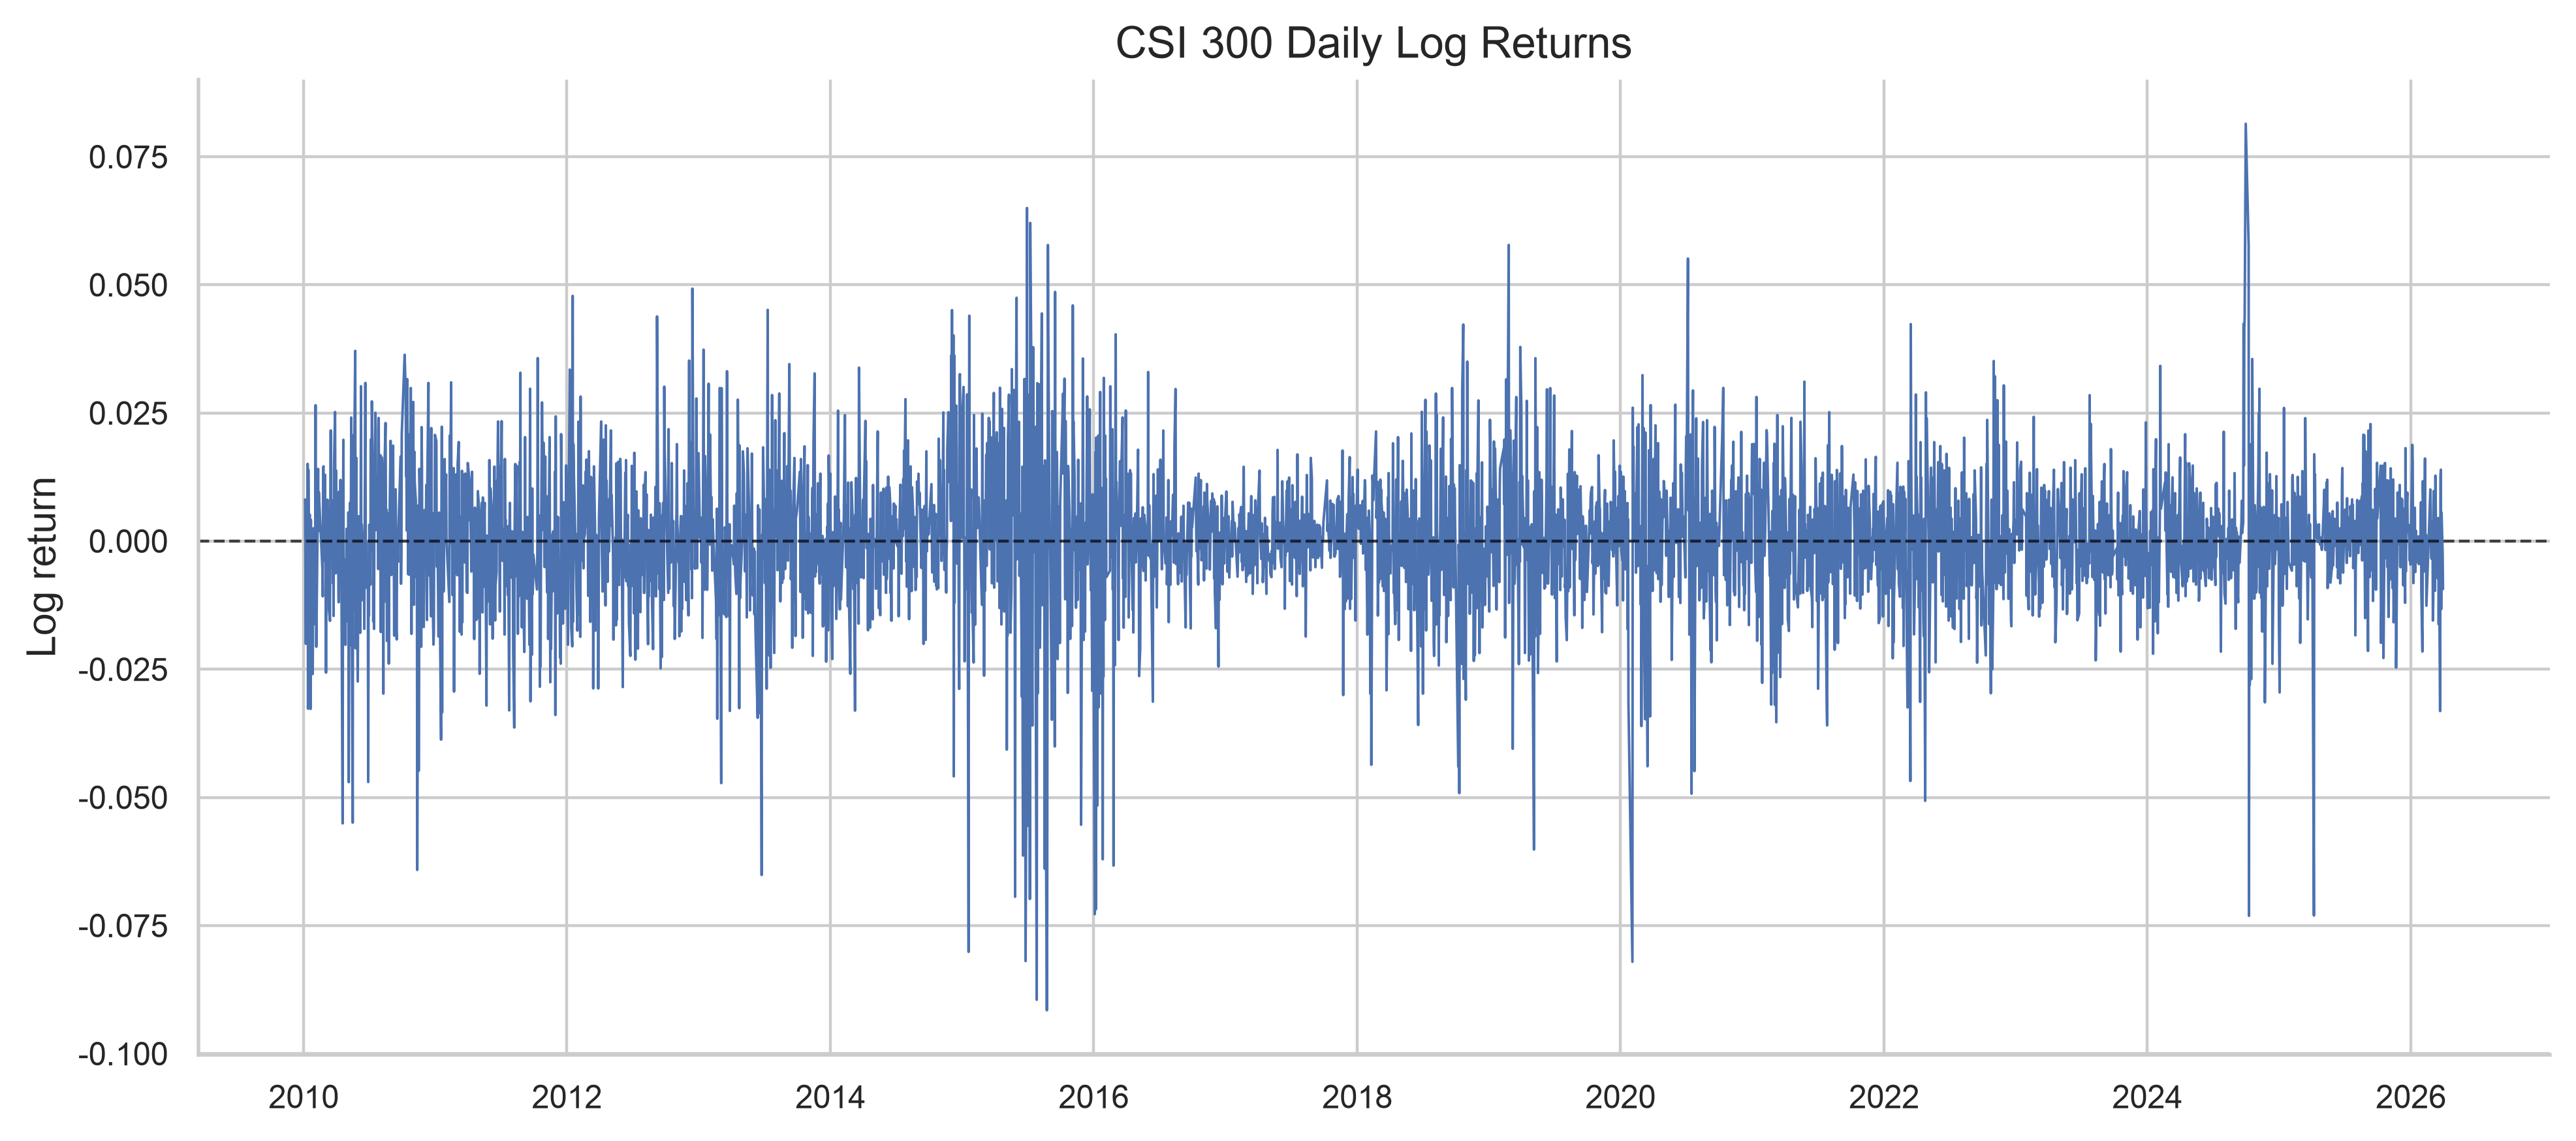
\includegraphics[width=.94\textwidth]{../../results/descriptive-corrected/figure_1_log_return_series.png}\\[0.5em]
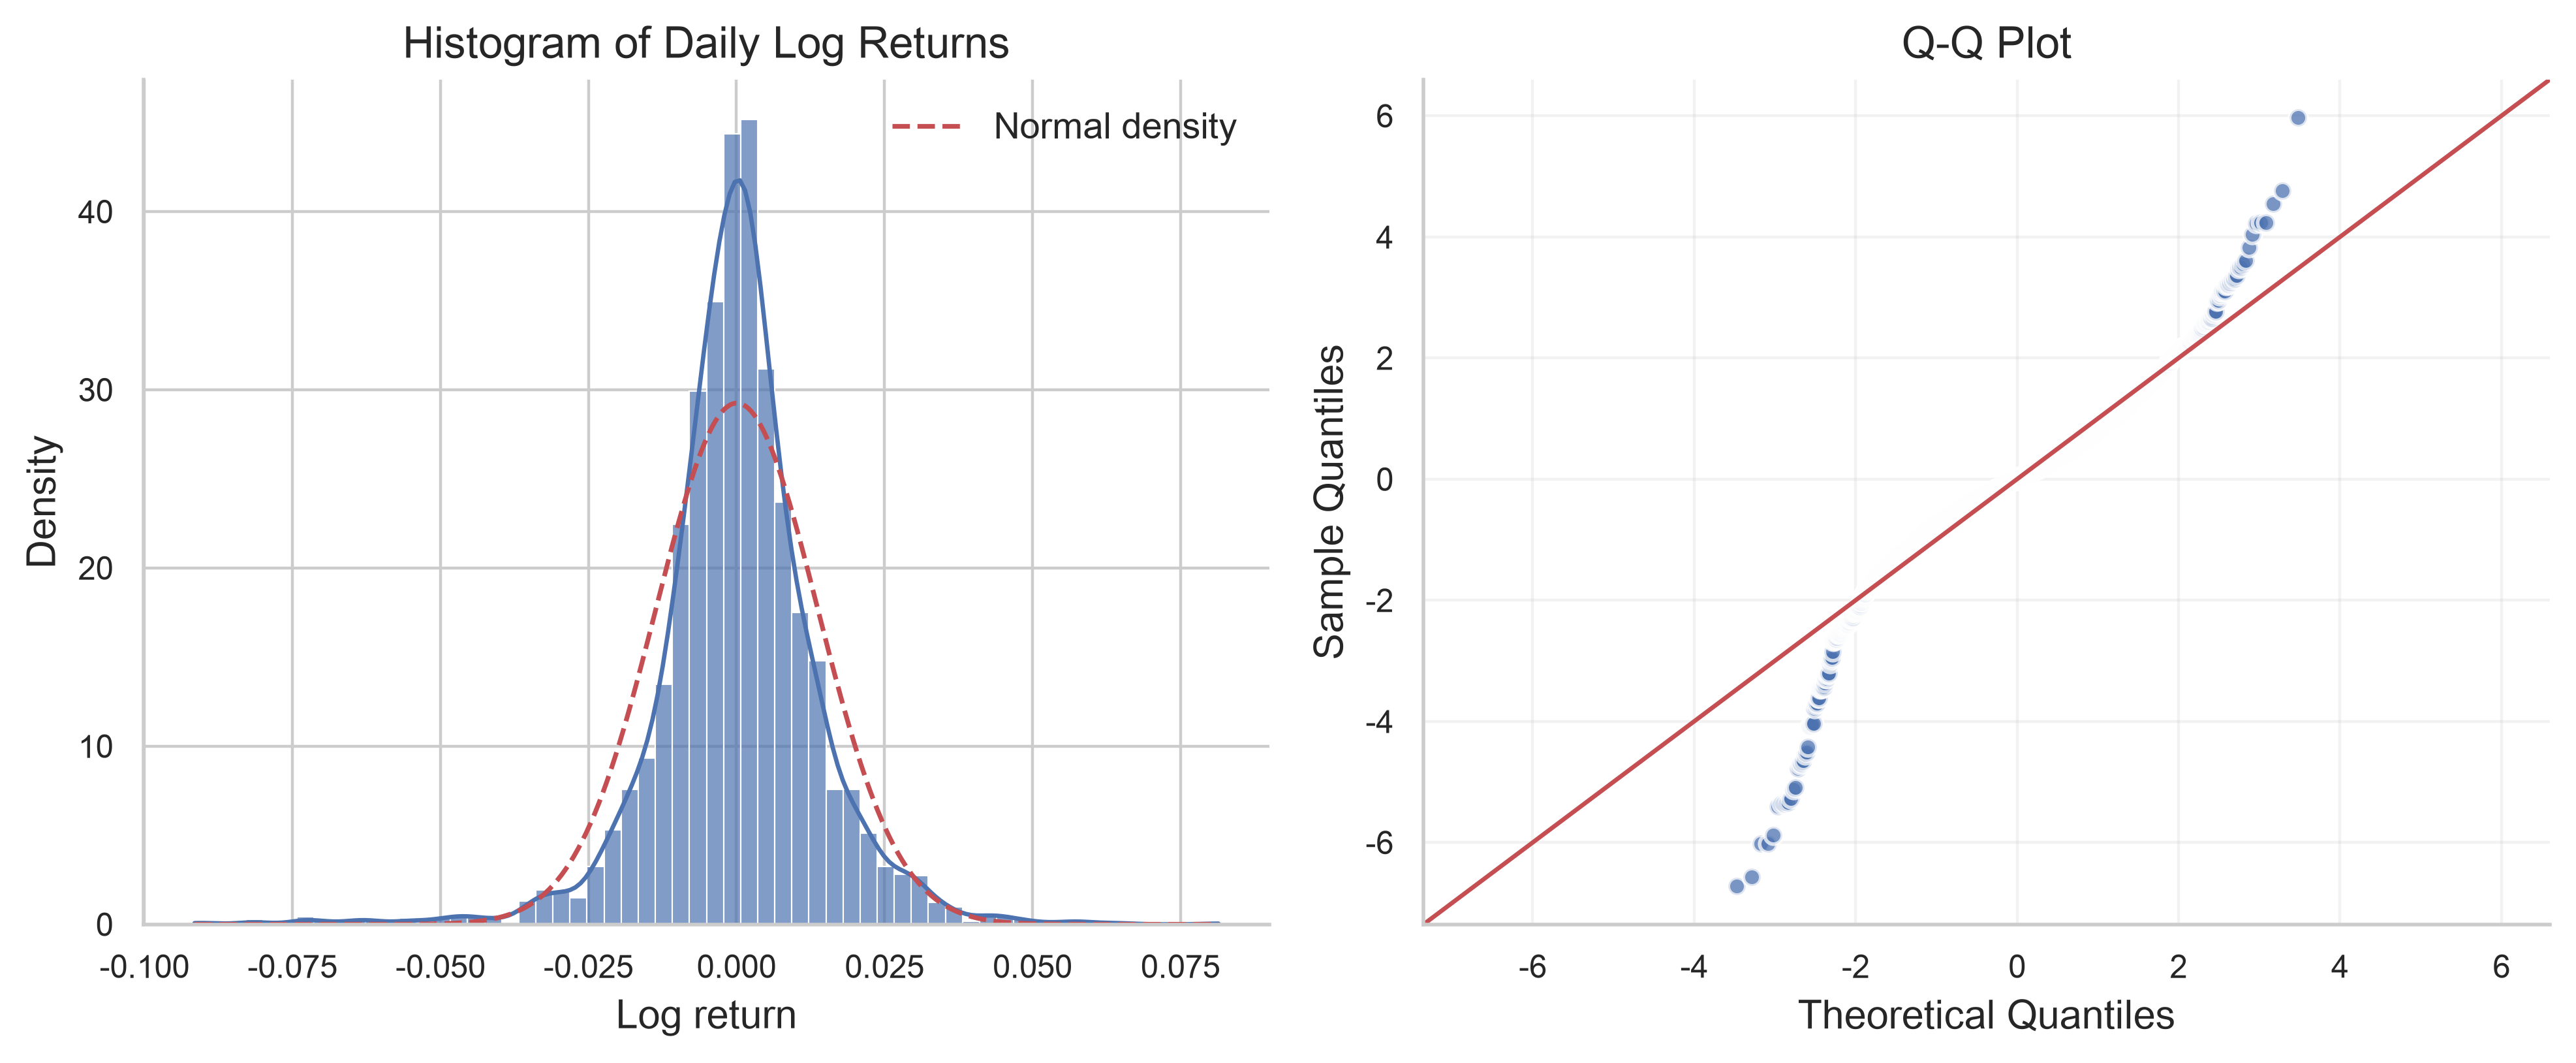
\includegraphics[width=.94\textwidth]{../../results/descriptive-corrected/figure_2_histogram_qq.png}
\caption{Corrected CSI300 return series, distribution, and normal quantile comparison.}
\label{fig:return_ts_qq}
\end{figure}

\subsection{Market-only baselines}
The HAR-style regression is estimated by ordinary least squares:
\begin{equation}
y_{t+1}=\beta_0+\beta_d\log(RV_t+\varepsilon)
+\beta_w\log(\overline{RV}_{t,5}+\varepsilon)
+\beta_m\log(\overline{RV}_{t,22}+\varepsilon)+u_{t+1},
\end{equation}
where $\overline{RV}_{t,h}=h^{-1}\sum_{j=0}^{h-1}RV_{t-j}$. This uses multiscale persistence but not intraday realized variance.

The GARCH benchmark has a zero conditional mean and standardized Student-$t$ innovations:
\begin{equation}
r_t=\epsilon_t=\sqrt{h_t}z_t,\qquad
h_t=\omega+\alpha\epsilon_{t-1}^2+\beta h_{t-1}.
\end{equation}
Under the usual nonnegative parameter restrictions, $\alpha+\beta<1$ is the familiar finite-second-moment stationarity condition. The forecast enters the log-target comparison as $\log(\widehat h_{t+1|t}+\varepsilon)$. EGARCH, GJR-GARCH, and realized-volatility extensions are not included, so this is a limited benchmark comparison.

XGB-Market uses nine predictors in the fixed order shown in Table~\ref{tab:variables_main}. It is fitted to the log target. No winsorization, standardization, or early stopping is used in the matched historical configuration. Important parameters are 300 trees, depth 4, learning rate 0.05, minimum child weight 3, row and column sampling fractions 0.8, $L_1$ regularization 0.1, and $L_2$ regularization 1. The CPU histogram algorithm, 256 bins, and seed 2026 are fixed. Appendix~\ref{app:training} provides the numerical reproduction qualifications.

\begin{table}[htbp]\centering\small
\caption{XGB-Market predictors, in matrix order. $H_t$, $L_t$, and $V_t$ are daily high, low, and volume.}
\label{tab:variables_main}
\begin{tabularx}{\textwidth}{lX}\toprule Code name & Definition\\\midrule
\texttt{log\_rv1} & $\log(RV_t+\varepsilon)$\\
\texttt{log\_rv5} & $\log(\overline{RV}_{t,5}+\varepsilon)$\\
\texttt{log\_rv22} & $\log(\overline{RV}_{t,22}+\varepsilon)$\\
\texttt{ret\_pos} & $\max(r_t,0)$\\
\texttt{ret\_neg} & $\min(r_t,0)$\\
\texttt{range\_log} & $\log(H_t/L_t)$\\
\texttt{range\_log\_5} & Five-observation average of $\log(H/L)$\\
\texttt{log\_volume} & $\log(V_t)$\\
\texttt{dlog\_volume} & $\log(V_t)-\log(V_{t-1})$\\\bottomrule
\end{tabularx}
\end{table}

HAR, GARCH, and XGBoost are re-estimated every 20 retained observations using expanding histories. The phrase ``every 20'' is a refit frequency, not a fixed rolling training-window length or a calendar-day interval. At an origin after the daily close, all target observations used for training must already have been realized. Filtering can make adjacent retained rows differ from adjacent exchange trading days; the timing audit therefore distinguishes row order from actual dates.

\subsection{MIDAS signal and dynamic error correction}
Let $m(t)$ be the calendar month containing forecast origin $t$. The EPU signal uses the preceding $K$ months:
\begin{equation}
s_t(\theta)=\sum_{k=1}^{K}w_k(\theta)\log(EPU_{m(t)-k}),
\qquad w_k\geq0,\quad\sum_{k=1}^K w_k=1.
\end{equation}
This convention excludes the current calendar month's value, but without vintage data it remains a retrospective lag convention rather than verified real-time availability.

For Beta weights, set $x_k=(K-k+1)/(K+1)$ and use
\begin{equation}
a_k=\max\{x_k^{\theta_1-1}(1-x_k)^{\theta_2-1},10^{-12}\},
\qquad w_k=a_k/\textstyle\sum_j a_j.
\end{equation}
For exponential Almon weights, set $z_k=(K-k+1)/K$ and use
\begin{equation}
w_k=\frac{\exp(\theta_1z_k+\theta_2z_k^2)}
{\sum_j\exp(\theta_1z_j+\theta_2z_j^2)}.
\end{equation}
The definitions and orientation of the lag index are part of the specification; a differently ordered lag vector would describe a different signal.

Define the realized first-stage forecast error as $e_t=y_t-\widehat y^{\mathrm{XGB}}_{t|t-1}$. These are sequential forecast errors, not residuals from a first stage fitted to the same target observations. DEC estimates
\begin{equation}
e_{t+1}=a+\rho e_t+\gamma s_t(\theta)+u_{t+1},
\label{eq:error_correction}
\end{equation}
and adds the fitted correction to the XGB-Market forecast. The lagged error is available after the origin's close. Since regressors depend on estimated first-stage forecasts, ordinary regression coefficients and standard errors do not automatically justify structural interpretations \citep{Pagan1984}.

The residual-only comparator, XGB-AR, instead fits $e_{t+1}=a+\rho e_t+u_{t+1}$ by OLS with the same available residual history and 60-observation refit frequency. It has no additional tuning search. Comparing DEC with XGB-AR isolates the predictive contribution of the added EPU component more directly than comparing DEC only with uncorrected XGBoost; it still does not identify causality.

\subsection{Stable profiled estimation and selection}
For a given lag family and $K$, write the lagged log-EPU matrix as $L$ and profile out the linear coefficients:
\begin{equation}
F(\theta)=\frac1n\min_{a,\rho,\gamma}
\|e-a\mathbf1-\rho e_{\mathrm{lag}}-\gamma Lw(\theta)\|^2.
\end{equation}
An SVD projection removes the intercept and lagged-error directions. This follows the variable-projection principle for separable nonlinear least squares \citep{GolubPereyra1973}. At a differentiable point of fixed rank, with profiled residual vector $r$,
\begin{equation}
\nabla_\theta F=-\frac{2\widehat\gamma}{n}
\left(L\frac{\partial w}{\partial\theta}\right)^{\!\top}r.
\end{equation}
The derivative accounts for weight normalization. For the clipped Beta numerator, the derivative is zero below the floor; its boundary is a kink, so smoothness must not be asserted everywhere.

Beta parameters are bounded in $[0.05,20]^2$ and use 25 starts from $\{0.05,0.5,1.5,5,20\}\times\{0.05,0.5,2,5,20\}$. Exponential Almon parameters are bounded in $[-5,5]^2$ and use the 25 Cartesian starts from $\{-5,-2.5,0,2.5,5\}^2$ plus the legacy start $(-0.2,-0.02)$. L-BFGS-B uses \texttt{ftol=1e-14}, \texttt{gtol=1e-9}, \texttt{maxiter=2000}, \texttt{maxfun=10000}, and \texttt{maxls=50}. These are numerical stopping controls, not statistical confidence thresholds. The projected gradient is checked against $10^{-6}$ for the mean-SSE objective; candidates failing this check are retried with SLSQP. Selection uses the lowest training objective. If the selected solution still fails stationarity acceptance, execution raises an error rather than selecting a convenient test-loss result. The solver terminology follows the documented optimizer interfaces.\footnote{SciPy L-BFGS-B reference: \url{https://docs.scipy.org/doc/scipy/reference/optimize.minimize-lbfgsb.html}.}

Each of the two lag families is evaluated at $K\in\{6,12,24\}$. The 500 first-stage validation observations supply 499 lagged residual pairs: the first 299 fit the second stage, and the remaining 200 score it by MSE in chronological order. The scoring segment uses newly available lagged errors but does not refit second-stage parameters within that segment. The selected family and $K$ remain fixed in the test period, while shape and linear coefficients are re-estimated every 60 retained observations using expanding information.

These rules were fixed before the current revised test results were computed. However, historical test behavior had already been examined. The study is therefore a retrospective reanalysis, not a preregistered test or an untouched holdout evaluation. Multistart search and small projected gradients provide stronger numerical evidence than a single success flag, but do not prove global optimality.

\subsection{Point losses and exploratory inference}
For $N$ common test observations,
\begin{align}
\mathrm{MSE}&=N^{-1}\sum_t(y_t-\widehat y_t)^2,\\
\mathrm{MAE}&=N^{-1}\sum_t|y_t-\widehat y_t|,\\
\mathrm{QLIKE}&=N^{-1}\sum_t\left[
\frac{RV_t}{\widehat{RV}_t}-\log\!\left(\frac{RV_t}{\widehat{RV}_t}\right)-1\right].
\end{align}
QLIKE is computed after the inverse transformation, with both proxy and forecast floored at $10^{-12}$. Lower values are better for all three losses. Proxy-robust ranking arguments require conditional-unbiasedness assumptions \citep{Patton2011}; the squared-return proxy, log offset, and floors should not be treated as automatically satisfying every such assumption.

For benchmark $A$, define $d_t=L_{A,t}-L_{\mathrm{DEC},t}$, so a positive mean favors DEC. Standard errors use the Newey--West Bartlett estimator \citep{NeweyWest1987} with bandwidth $\lfloor4(N/100)^{2/9}\rfloor$, equal to 7 for these samples. Two-sided normal-tail probabilities are computed with a survival function to avoid numerical zeros. Holm adjustment is applied jointly to 18 comparisons: three markets, three losses, and two XGB benchmarks \citep{Holm1979}.

These are exploratory loss-difference diagnostics. Estimated and nested models, generated regressors, validation selection, expanding estimation, and prior exposure to results limit a conventional confirmatory interpretation. The legacy Clark--West calculation used an ordinary standard error and a one-sided $t$ calculation; it is not retained as current evidence of a confirmatory forecasting advantage. No test outcome establishes a causal EPU channel.

\subsection{Rolling-residual prediction intervals}
For each model, calibrate using past absolute log-target forecast errors. With $n$ available errors, at least 60 are required. The window is $m\in\{120,250,500\}$, and nominal miscoverage is $\alpha\in\{0.10,0.05\}$. The radius is the ordered error at rank $\lceil(n+1)(1-\alpha)\rceil$. The code caps a rank above $n$ at the largest observed error; that branch is not triggered by the reported settings and supplies no universal finite-sample guarantee.

The log interval is $[\widehat y-q,\widehat y+q]$. If transformed back, bounds are $\max\{0,\exp(\widehat y\mp q)-\varepsilon\}$. Reported width and interval scores below are on the log-target scale. For log bounds $L_t,U_t$,
\begin{equation}
IS_\alpha(L_t,U_t;y_t)=U_t-L_t+
\frac{2}{\alpha}(L_t-y_t)\mathbf1\{y_t<L_t\}+
\frac{2}{\alpha}(y_t-U_t)\mathbf1\{y_t>U_t\}.
\end{equation}
Empirical coverage, mean width, and mean interval score are evaluated jointly. Narrower intervals alone are not necessarily better. With serial dependence, changing distributions, and unverified real-time EPU availability, this calibration rule should not be presented as an exchangeability-based coverage guarantee. It is not EnbPI, and the intervals describe a future observed proxy, not confidence intervals for latent conditional variance.

\section{CSI300 point forecasts and residual ablation}
\label{sec:point}
The current CSI300 test contains 1919 forecast origins from 2018-05-03 to 2026-03-30. Results in this section come from \path{results/revised/}. XGBoost uses the configuration and sampling behavior that matched the archived predictions; the current reanalysis reuses the verified first-stage cache, with dates, targets, flags, and hashes checked. HAR, GARCH, DEC, and XGB-AR are re-estimated. Historical outputs remain separate rather than being overwritten.

\subsection{Loss comparisons}
\begin{table}[htbp]\centering
\caption{Revised CSI300 point losses, $N=1919$. MSE and MAE use the log target.}
\label{tab:forecast_metrics}
\begin{tabular}{lrrr}\toprule Model & MSE & MAE & QLIKE\\\midrule
HAR & 4.905206 & 1.724860 & 3.905553\\
GARCH(1,1) & 7.375868 & 1.983865 & 1.564183\\
XGB-Market & 5.099716 & 1.763086 & 4.951636\\
XGB-AR & 5.094169 & 1.758021 & 4.705936\\
DEC & 5.112644 & 1.725558 & 3.536964\\\bottomrule
\end{tabular}
\end{table}

HAR has the lowest log-MSE and MAE, whereas GARCH has the lowest QLIKE. Relative to XGB-Market, DEC reduces QLIKE by approximately 28.57\% and MAE by 2.13\%, but increases MSE by 0.25\%. Thus, the more elaborate correction does not dominate the simpler baselines across losses. Part of the ranking difference reflects the distinction between log-target fitting and direct conditional-variance modeling.

Against XGB-AR, DEC lowers QLIKE from 4.705936 to 3.536964 and MAE from 1.758021 to 1.725558, while raising MSE from 5.094169 to 5.112644. This is a loss-dependent incremental comparison for the EPU component. It does not demonstrate an exogenous policy-uncertainty effect or prove that the monthly inputs were available in real time.

\begin{figure}[htbp]\centering
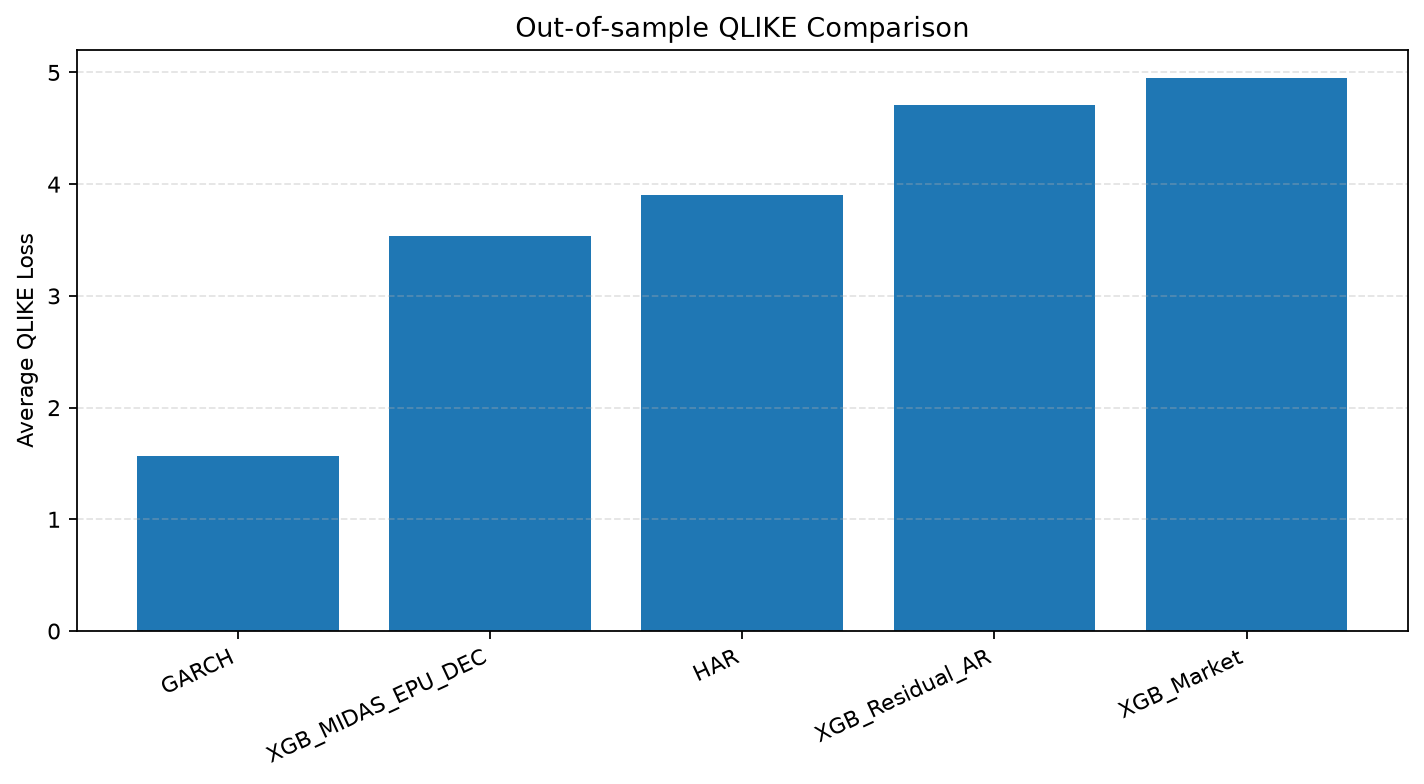
\includegraphics[width=.9\textwidth]{../../results/revised/csi300/fig_metrics_bar.png}
\caption{Revised CSI300 QLIKE across the five models. Lower is better.}
\label{fig:metrics_bar}
\end{figure}

\subsection{Forecast paths and cumulative losses}
Figures~\ref{fig:prediction_series} and~\ref{fig:cumulative_qlike} show recent forecasts and cumulative QLIKE differences. The latter cumulates benchmark loss minus DEC loss. An increase therefore moves the comparison in DEC's favor, but does not show that DEC improves every date or rule out concentration in extreme observations. A smoother prediction path is not by itself evidence of forecasting validity.

\begin{figure}[htbp]\centering
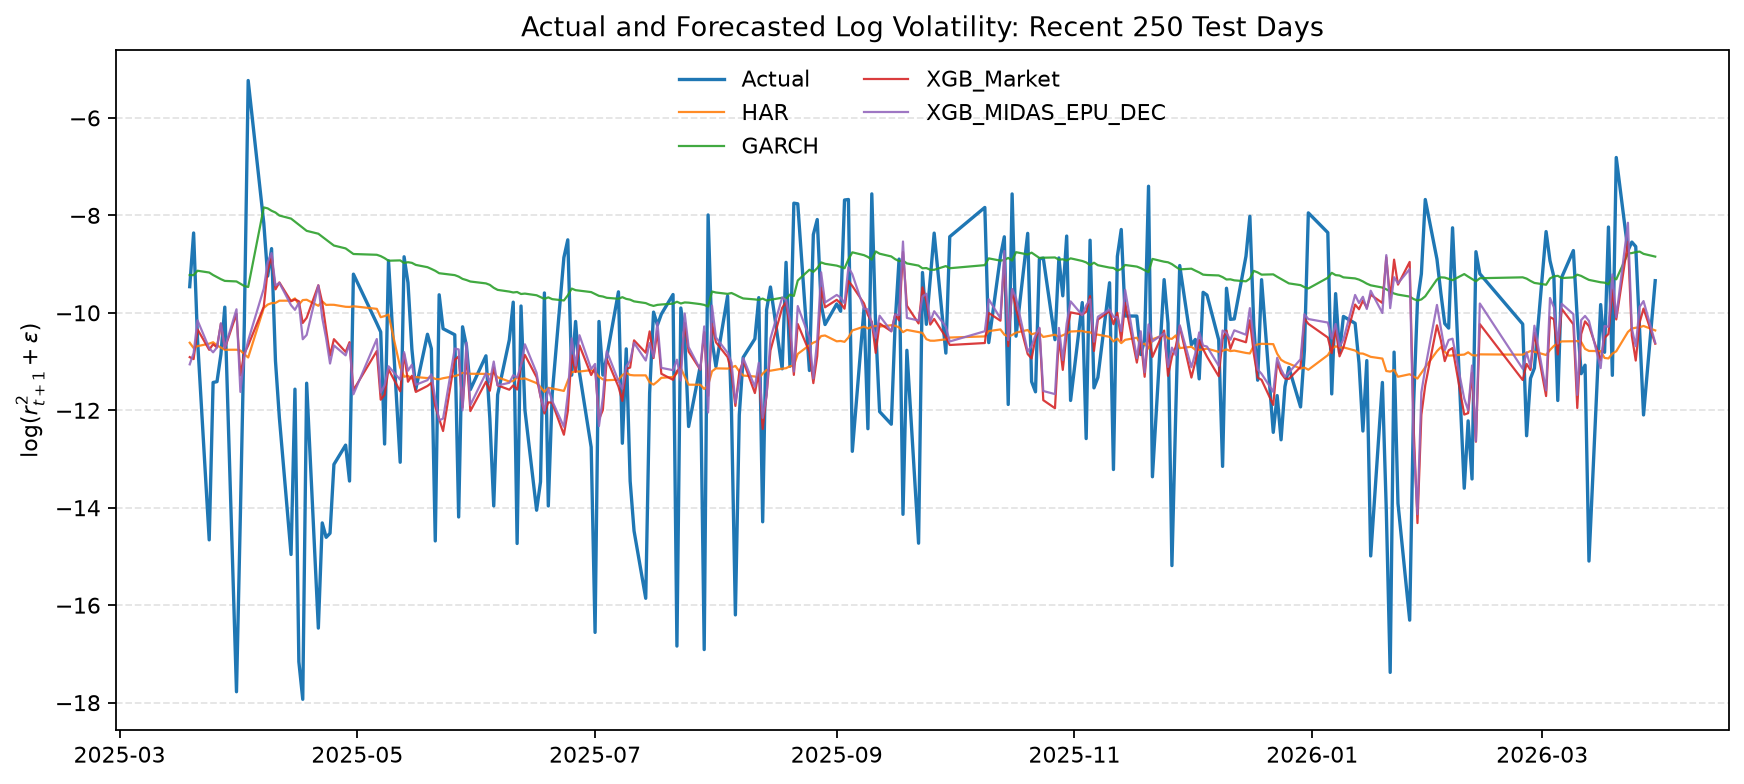
\includegraphics[width=.9\textwidth]{../../results/revised/csi300/fig_prediction_series_recent.png}
\caption{Recent revised DEC forecasts and three market-model benchmarks.}
\label{fig:prediction_series}
\end{figure}
\begin{figure}[htbp]\centering
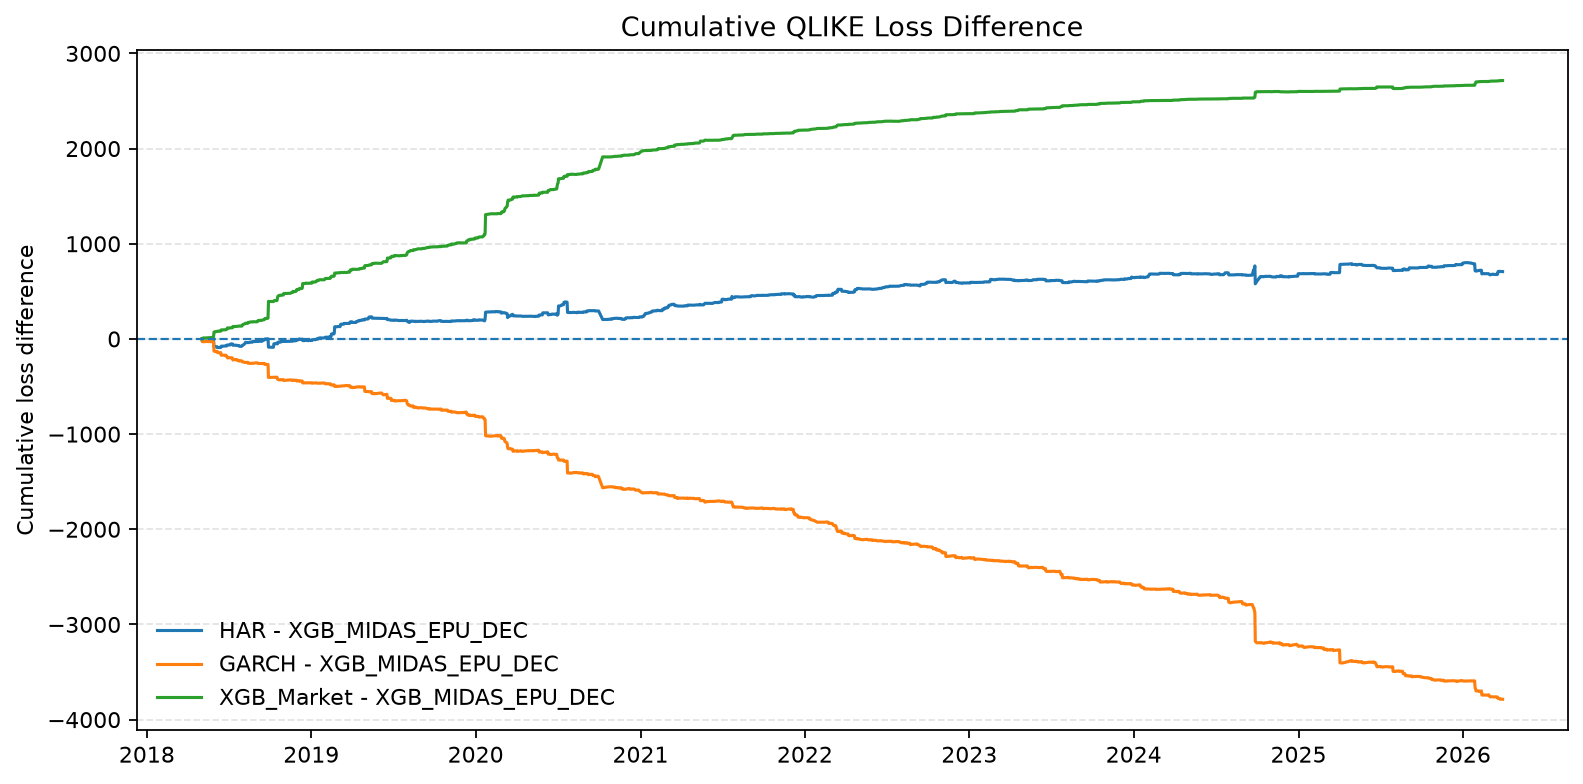
\includegraphics[width=.9\textwidth]{../../results/revised/csi300/fig_cumulative_qlike_diff.png}
\caption{Cumulative CSI300 QLIKE differences: benchmark minus revised DEC.}
\label{fig:cumulative_qlike}
\end{figure}

\subsection{Exploratory loss-difference diagnostics}
Table~\ref{tab:hypothesis_tests} reports the six CSI300 comparisons within the joint 18-comparison Holm adjustment. The reference calculations provide evidence of lower sample MAE and QLIKE relative to the two XGB benchmarks, but not of lower MSE. Their interpretation remains exploratory because of selection, approximate nesting, estimated forecasts, and the retrospective design.

\begin{table}[htbp]\centering\small
\caption{Exploratory CSI300 HAC diagnostics. Positive differences favor DEC.}
\label{tab:hypothesis_tests}
\begin{tabular}{llrrr}\toprule Benchmark & Loss & Mean difference & HAC SE & Holm $p$\\\midrule
XGB-Market & MSE & $-0.012928$ & 0.041430 & 1\\
XGB-Market & MAE & 0.037528 & 0.008207 & $6.73\times10^{-5}$\\
XGB-Market & QLIKE & 1.414672 & 0.197725 & $1.43\times10^{-11}$\\
XGB-AR & MSE & $-0.018475$ & 0.035984 & 1\\
XGB-AR & MAE & 0.032464 & 0.007137 & $7.01\times10^{-5}$\\
XGB-AR & QLIKE & 1.168972 & 0.160859 & $6.61\times10^{-12}$\\\bottomrule
\end{tabular}
\end{table}

\subsection{Selected weights and numerical sensitivity}
CSI300 retains a 24-month exponential Almon specification. Table~\ref{tab:midas_spec} and Figure~\ref{fig:midas_weights} describe the validation-stage choice; test-period parameters are subsequently re-estimated every 60 retained observations. The boundary value of $\theta_1$ indicates that the fitted shape depends on the imposed parameter constraints. These weights should not be interpreted as a stable causal policy-transmission profile.

\begin{table}[htbp]\centering
\caption{CSI300 specification selected by validation MSE.}
\label{tab:midas_spec}
\begin{tabular}{lrrrr}\toprule Family & $K$ & $\theta_1$ & $\theta_2$ & Validation MSE\\\midrule
Exponential Almon & 24 & 5.000000 & $-4.488853$ & 5.722685\\\bottomrule
\end{tabular}
\end{table}
\begin{figure}[htbp]\centering
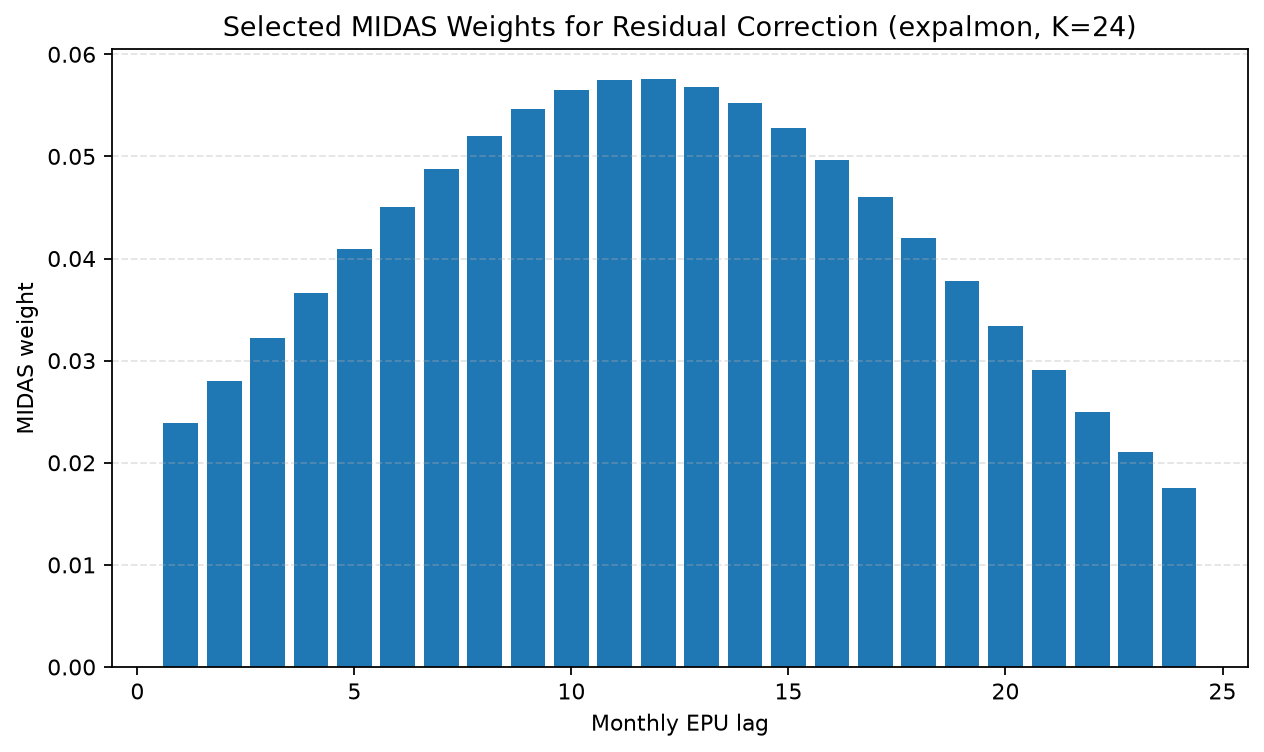
\includegraphics[width=.9\textwidth]{../../results/revised/csi300/fig_midas_weights.png}
\caption{CSI300 MIDAS weights from revised validation selection.}
\label{fig:midas_weights}
\end{figure}

Archived DEC has MSE 5.112383 and QLIKE 3.538317, compared with 5.112644 and 3.536964 after revision. MSE is slightly worse and QLIKE slightly better. The reason for revising the solver is the documented estimation defect and improved numerical diagnostics, not a desire to select the most favorable test scores. Appendix~\ref{app:solver} separates historical reproduction differences from current-method stability checks.

\section{CSI300 rolling-residual prediction intervals}
\label{sec:intervals}
Point-loss improvements need not improve interval forecasts. This section applies the same absolute-residual construction to all five models and evaluates the 30 combinations of model, nominal coverage, and calibration window described in Section~\ref{sec:methods}. Width and interval score are reported on the log-target scale.

\subsection{A common evaluation sample}
DEC and XGB-AR do not have corrected predictions in the first-stage validation segment, so they first accumulate 60 realized test residuals. All settings are then evaluated on the same 1859 dates, from 2018-07-27 to 2026-03-30. Other models may still use their available validation residuals for calibration: common evaluation dates do not require discarding information that would already have been available to a model. All interval figures and coverage diagnostics use this same evaluation sample.

\begin{table}[htbp]\centering
\caption{Common-date 90\% intervals with calibration window 250.}
\label{tab:interval_main}\label{tab:common_intervals}
\begin{tabular}{lrrrr}\toprule Model & $N$ & Coverage & Mean width & Mean score\\\midrule
HAR & 1859 & 0.9005 & 6.9949 & 9.6973\\
GARCH(1,1) & 1859 & 0.8967 & 9.1225 & 12.6634\\
XGB-Market & 1859 & 0.8983 & 7.0644 & 9.8534\\
XGB-AR & 1859 & 0.9021 & 7.0662 & 9.8793\\
DEC & 1859 & 0.8989 & 7.0634 & 10.1995\\\bottomrule
\end{tabular}
\end{table}

DEC's interval score is worse than those of HAR, XGB-Market, and XGB-AR, although better than GARCH's under this construction. Its interval is slightly narrower than those of the two XGB comparators, but that small width advantage does not offset the score penalties for misses. No significance test of interval-score differences is reported. The GARCH comparison concerns the same log-residual interval algorithm, not intervals derived directly from the model's conditional innovation distribution.

\begin{figure}[htbp]\centering
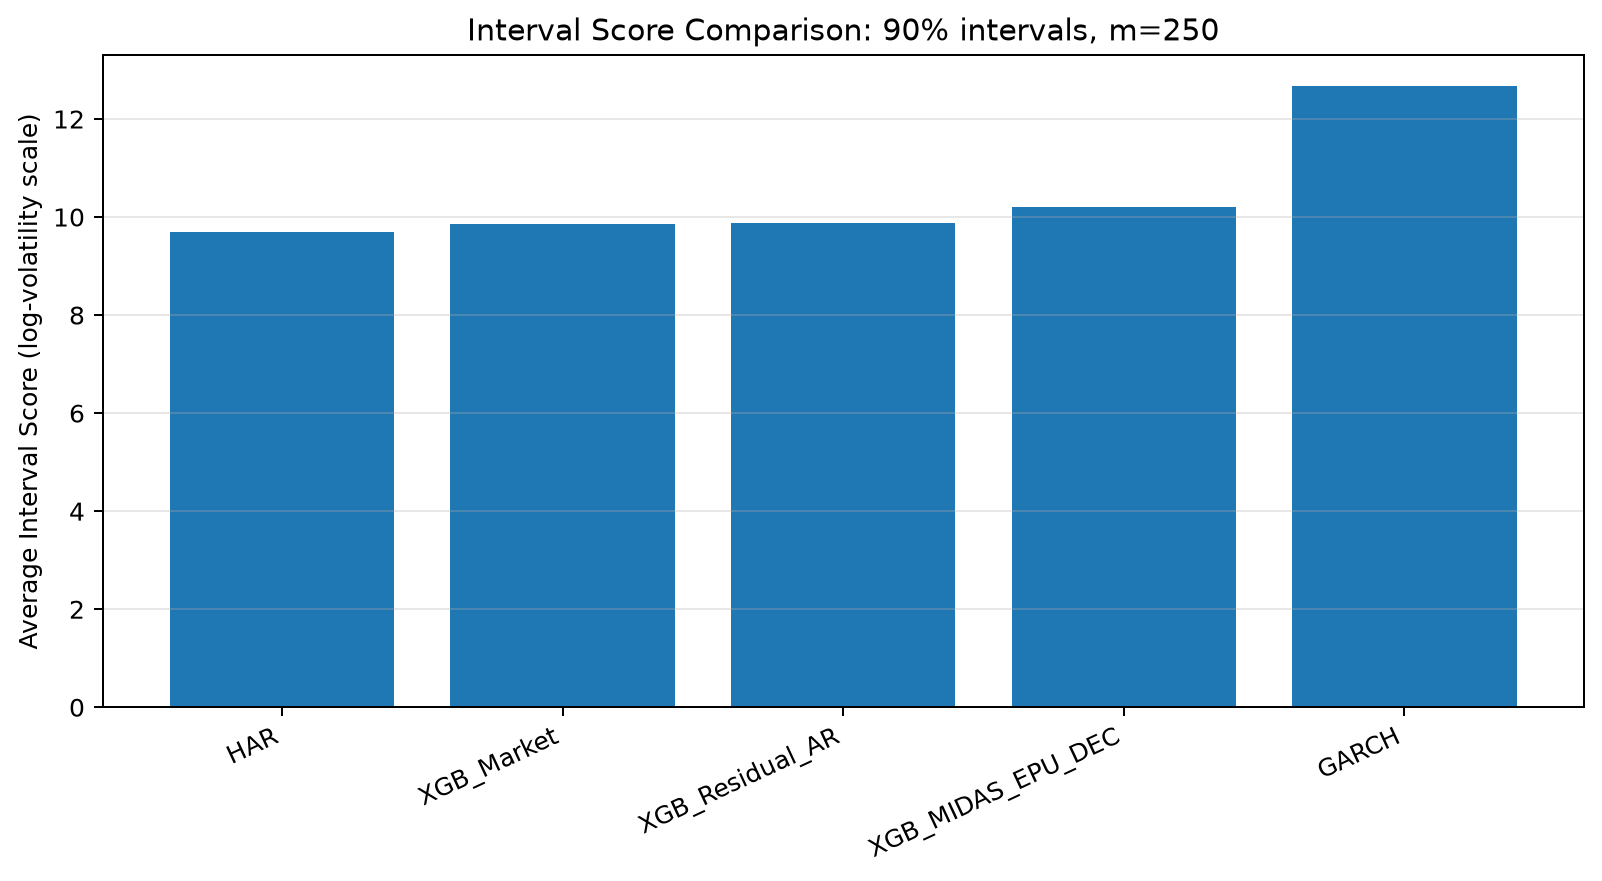
\includegraphics[width=.9\textwidth]{../../results/revised/intervals/fig_interval_score_main.png}
\caption{Mean interval scores on the common evaluation dates. Lower is better.}
\label{fig:interval_score_main}
\end{figure}
\begin{figure}[htbp]\centering
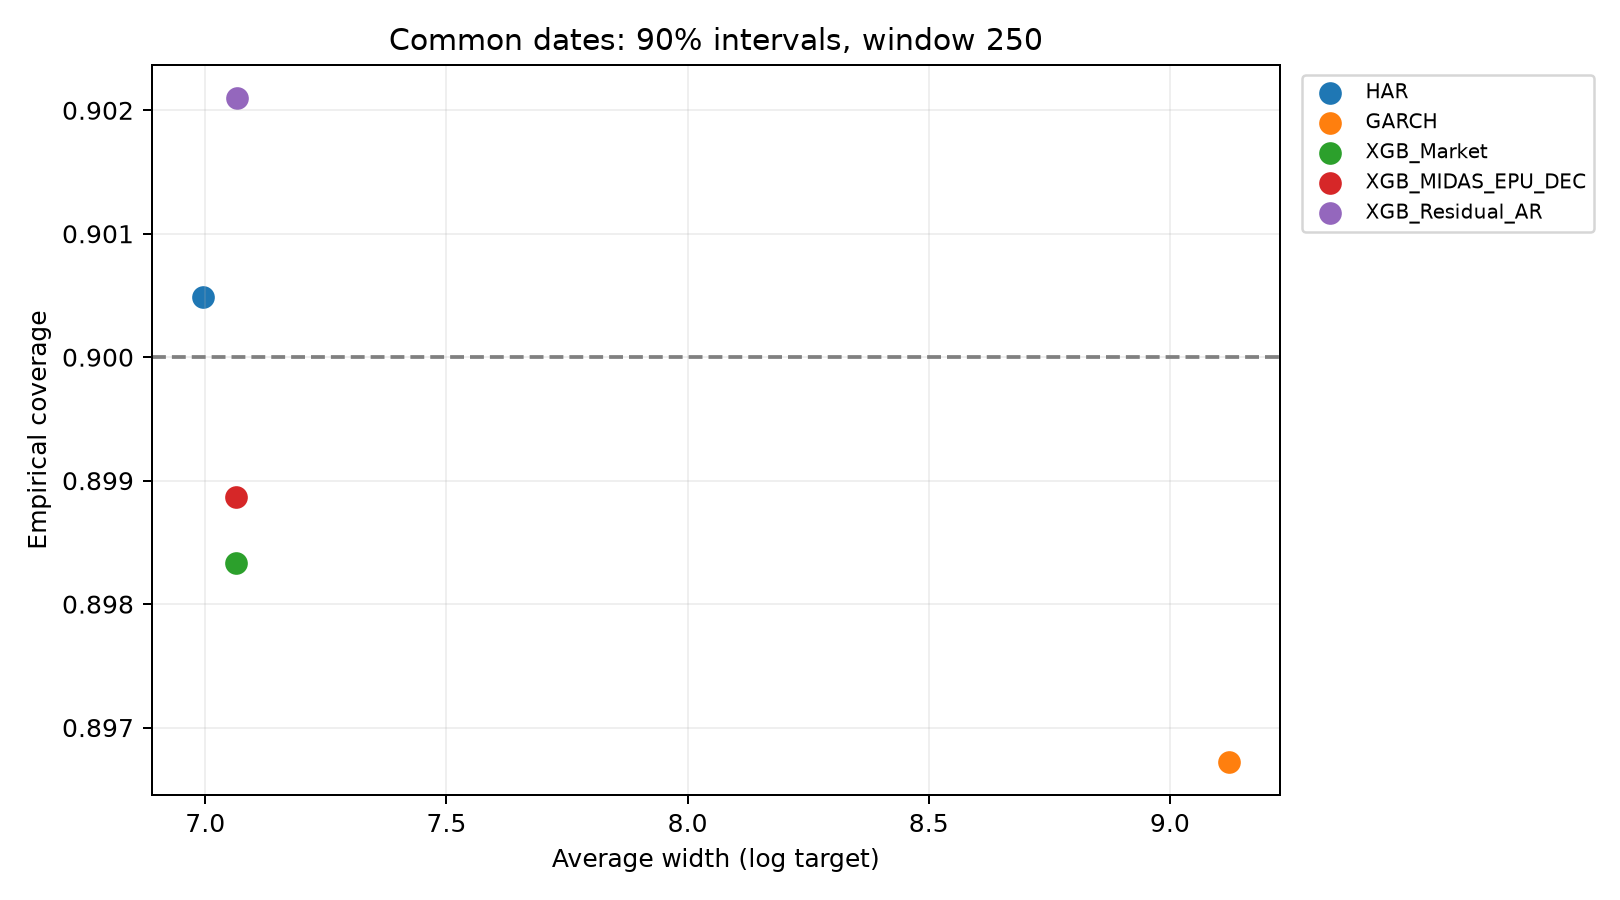
\includegraphics[width=.9\textwidth]{../../results/revised/intervals/fig_coverage_width_tradeoff_main.png}
\caption{Empirical coverage and mean width under the main setting.}
\label{fig:coverage_width_tradeoff}
\end{figure}

\subsection{Coverage diagnostics and temporal behavior}
Christoffersen-style diagnostics examine unconditional coverage (UC), independence of violations (IND), and joint conditional coverage (CC). For the main setting, none of the five models is rejected at the 5\% reference level (Table~\ref{tab:christoffersen_main}). Non-rejection is not proof of correct coverage, and these coverage diagnostics are not adjusted for multiple testing.

\begin{table}[htbp]\centering
\caption{Coverage diagnostics for the main common-date setting.}
\label{tab:christoffersen_main}
\begin{tabular}{lrrrr}\toprule Model & Violations & $p_{uc}$ & $p_{ind}$ & $p_{cc}$\\\midrule
HAR & 185 & 0.9445 & 0.1024 & 0.2629\\
GARCH(1,1) & 192 & 0.6388 & 0.1370 & 0.2964\\
XGB-Market & 189 & 0.8110 & 0.0987 & 0.2487\\
XGB-AR & 182 & 0.7623 & 0.1896 & 0.4041\\
DEC & 188 & 0.8712 & 0.0880 & 0.2303\\\bottomrule
\end{tabular}
\end{table}

The less favorable settings must also be retained. At 95\% nominal coverage with a window of 120, DEC has $p_{ind}=0.0062$ and $p_{cc}=0.0233$, indicating clustered violations under these reference diagnostics. A favorable aggregate coverage rate can conceal local failures.

Figure~\ref{fig:rolling_coverage} uses overlapping 60-observation windows; adjacent values are therefore not independent replications. The recent interval path in Figure~\ref{fig:interval_series_xgb_midas} is a descriptive view of sample behavior, not evidence that every miss is attributable to unforeseeable noise or a sudden shock.

\begin{figure}[htbp]\centering
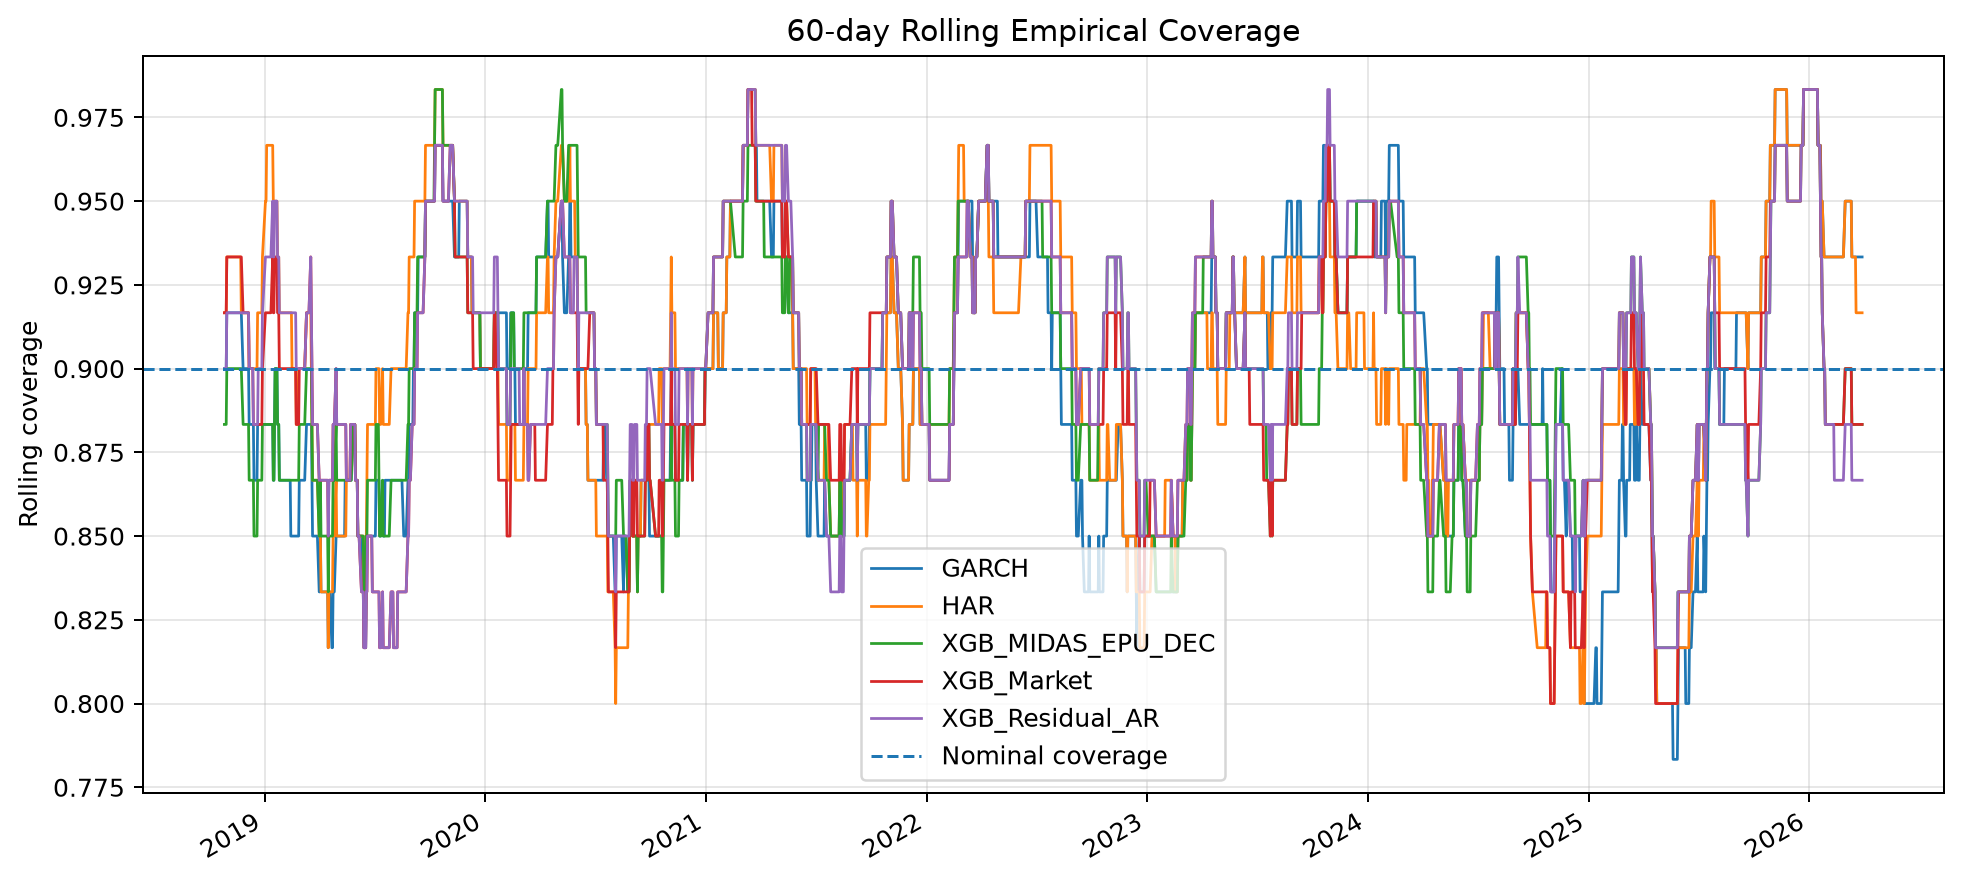
\includegraphics[width=.9\textwidth]{../../results/revised/intervals/fig_rolling_coverage_main.png}
\caption{Rolling coverage over 60 observations within the common evaluation period.}
\label{fig:rolling_coverage}
\end{figure}
\begin{figure}[htbp]\centering
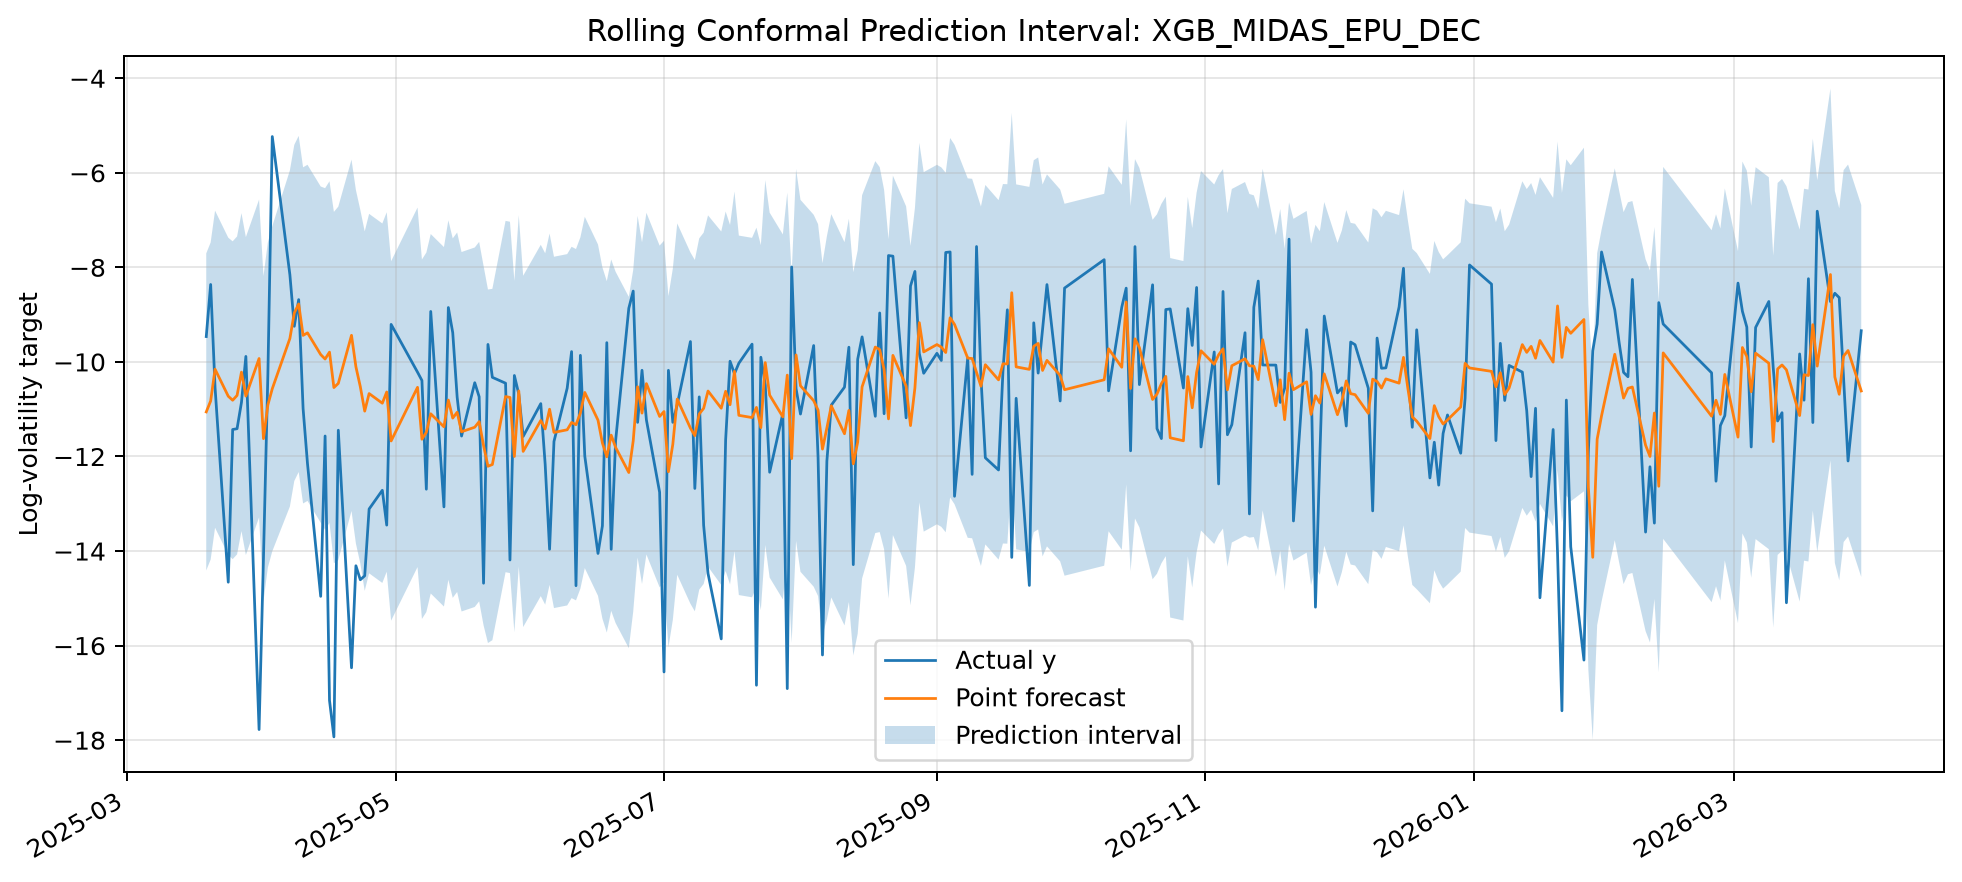
\includegraphics[width=.9\textwidth]{../../results/revised/intervals/fig_interval_series_XGB_MIDAS_EPU_DEC.png}
\caption{Recent revised DEC intervals from rolling absolute residuals.}
\label{fig:interval_series_xgb_midas}
\end{figure}

\subsection{Window sensitivity}
\begin{table}[htbp]\centering
\caption{Mean scores for 90\% intervals on the same 1859 dates.}
\label{tab:interval_robustness}
\begin{tabular}{lrrr}\toprule Model & Window 120 & Window 250 & Window 500\\\midrule
HAR & 9.7468 & 9.6973 & 9.6938\\
GARCH(1,1) & 12.6511 & 12.6634 & 12.6021\\
XGB-Market & 9.9336 & 9.8534 & 9.8528\\
XGB-AR & 9.9387 & 9.8793 & 9.8628\\
DEC & 10.2852 & 10.1995 & 10.1807\\\bottomrule
\end{tabular}
\end{table}

All 30 settings, including both nominal levels, are supplied in the accompanying results. Conclusions should be tied to the particular window and level, rather than generalized from the main setting alone. The main DEC score changes from the historical 10.1991 to 10.1995 after revision, a slight deterioration; the numerical correction does not reverse the benchmark conclusion.

For CSI300, lower QLIKE and better interval scores are distinct claims. The revised analysis does not support both simultaneously. These findings apply to the future observed proxy and this residual-based interval construction; they do not establish valid confidence intervals for latent variance.

\section{Revised results in alternative markets}
\label{sec:robustness}
SSE50 and the Nasdaq Composite provide comparisons under the same model families and residual ablation. Corrected SSE50 has train/validation/test counts of 1500/500/1919, whereas Nasdaq retains 2000/500/1554. SSE50 uses Chinese monthly EPU and Nasdaq uses US monthly EPU. Differences in markets and estimation lengths limit direct cross-market interpretation; neither sample is an untouched independent external validation set.

\subsection{Point losses}
\begin{table}[htbp]\centering
\caption{Calendar-corrected SSE50 point losses, $N=1919$.}
\label{tab:sse50_metrics}
\begin{tabular}{lrrr}\toprule Model & MSE & MAE & QLIKE\\\midrule
HAR & 4.826226 & 1.717026 & 3.872429\\
GARCH(1,1) & 7.537442 & 2.043060 & 1.586804\\
XGB-Market & 4.940740 & 1.740321 & 4.753901\\
XGB-AR & 4.954984 & 1.741490 & 4.697720\\
DEC & 4.972472 & 1.718639 & 3.672557\\\bottomrule
\end{tabular}
\end{table}
\begin{table}[htbp]\centering
\caption{Revised Nasdaq point losses, $N=1554$.}
\label{tab:nas_metrics}
\begin{tabular}{lrrr}\toprule Model & MSE & MAE & QLIKE\\\midrule
HAR & 5.292393 & 1.814872 & 3.994306\\
GARCH(1,1) & 7.110225 & 1.894212 & 1.498305\\
XGB-Market & 5.284620 & 1.767569 & 4.279836\\
XGB-AR & 5.302560 & 1.761263 & 4.224645\\
DEC & 5.369943 & 1.772158 & 3.895152\\\bottomrule
\end{tabular}
\end{table}

In SSE50, DEC improves QLIKE and MAE relative to both XGB comparators but worsens MSE. In Nasdaq, it improves QLIKE while worsening both MSE and MAE. Across all three markets, GARCH has the lowest QLIKE, followed by DEC. The gains associated with including EPU are therefore loss-dependent and do not imply general dominance.

\subsection{Why the Nasdaq specification changes}
The historical single-start 12-month Beta fit has training SSE approximately 1780.2771 on 299 residual pairs and validation MSE approximately 4.3325. Multistart estimation finds a lower training SSE of approximately 1779.2408, but its validation MSE increases to 5.0476. The 12-month exponential Almon candidate has validation MSE 4.3446 and is then selected among the six candidates. The switch follows the validation rule; it is not a choice based on favorable test QLIKE.

Fixing the historical 12-month Beta family while repairing only the solver produces Nasdaq test MSE 5.434646 and QLIKE 3.791512. Re-selecting by the stated validation rule produces MSE 5.369943 and QLIKE 3.895152. An inferior training optimum may have behaved like implicit regularization in this finite sample, but this is an explanatory hypothesis, not a reason to claim that the old optimizer correctly minimized its objective.

Archived DEC has MSE 5.423666 and QLIKE 3.794736. The selected revised Almon model therefore improves MSE by about 0.99\% while worsening QLIKE by about 2.65\%. Both changes must be reported. In SSE50, calendar correction and solver revision occur together, so the full difference from archived results cannot be attributed entirely to the optimizer. A separate calendar-control experiment is retained in Appendix~\ref{app:training}.

\subsection{Graphical comparisons}
The figures retain the same current-result images as the Chinese edition. Weight panels show the validation-stage selection, not invariant test-period coefficients. Both Chinese markets select 24-month exponential Almon weights; Nasdaq selects 12 months. Boundary solutions and re-estimation prevent a stable policy-transmission interpretation.

\begin{figure}[htbp]\centering
\begin{minipage}{.48\textwidth}\centering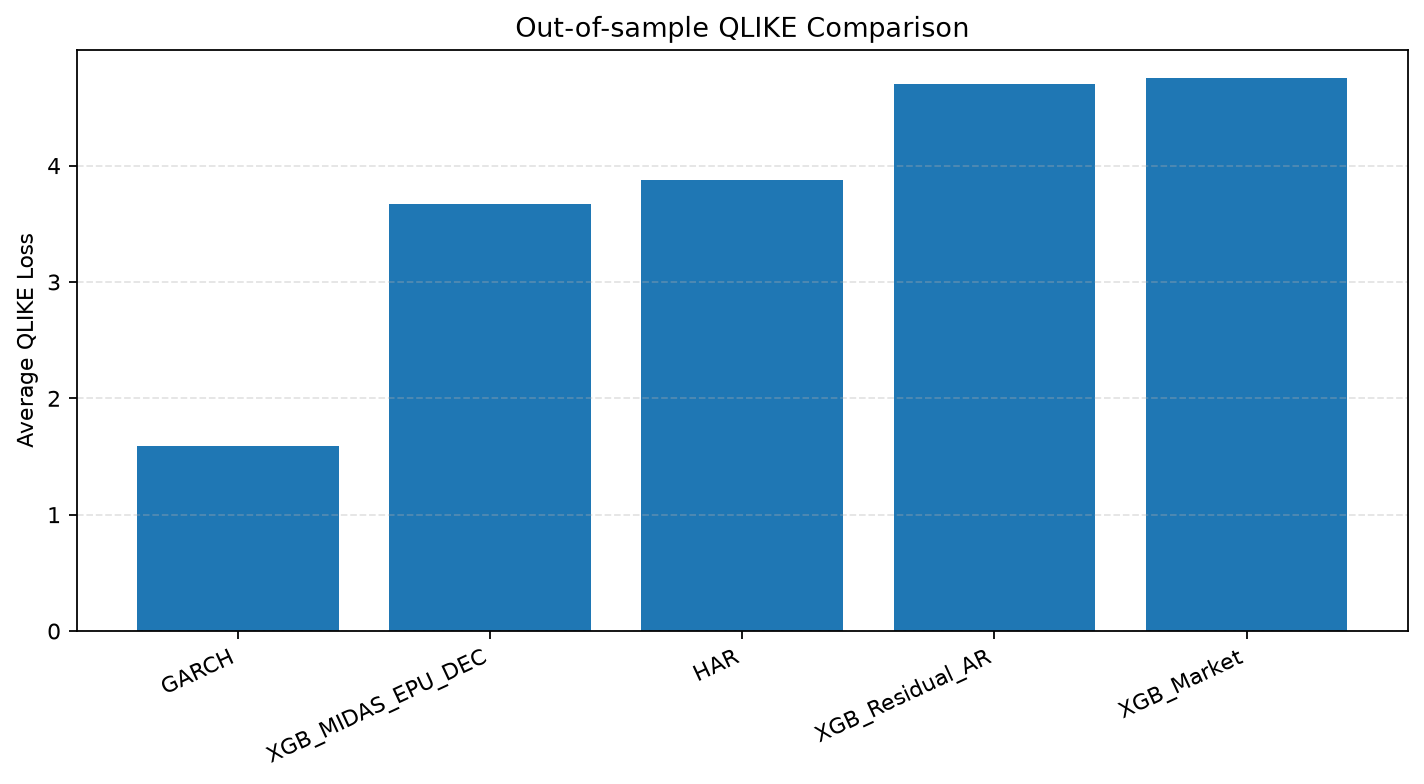
\includegraphics[width=\linewidth]{../../results/revised/sse50/fig_metrics_bar.png}\par{\small QLIKE}\end{minipage}\hfill
\begin{minipage}{.48\textwidth}\centering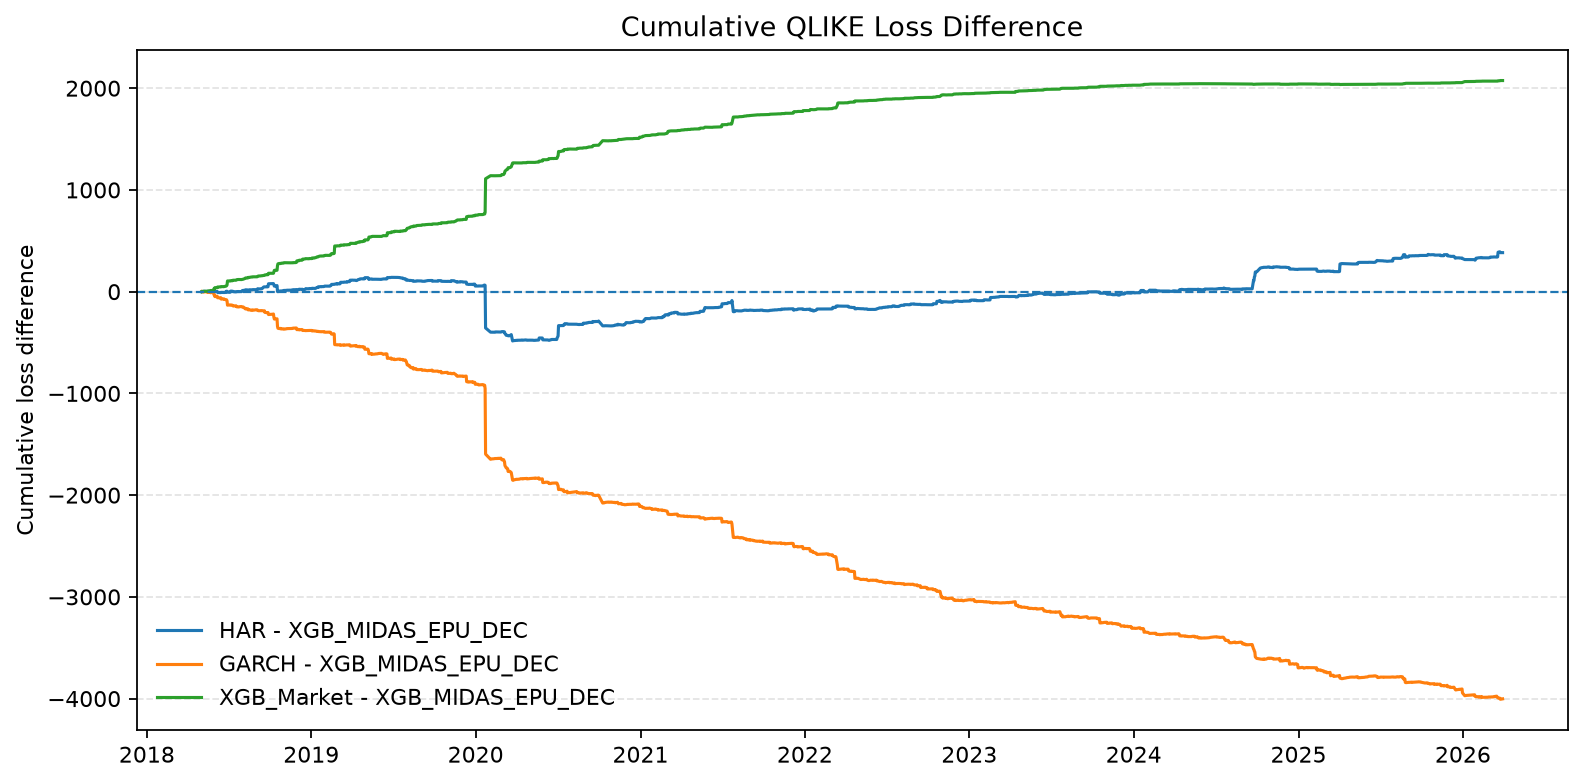
\includegraphics[width=\linewidth]{../../results/revised/sse50/fig_cumulative_qlike_diff.png}\par{\small Cumulative QLIKE differences}\end{minipage}\par\medskip
\begin{minipage}{.48\textwidth}\centering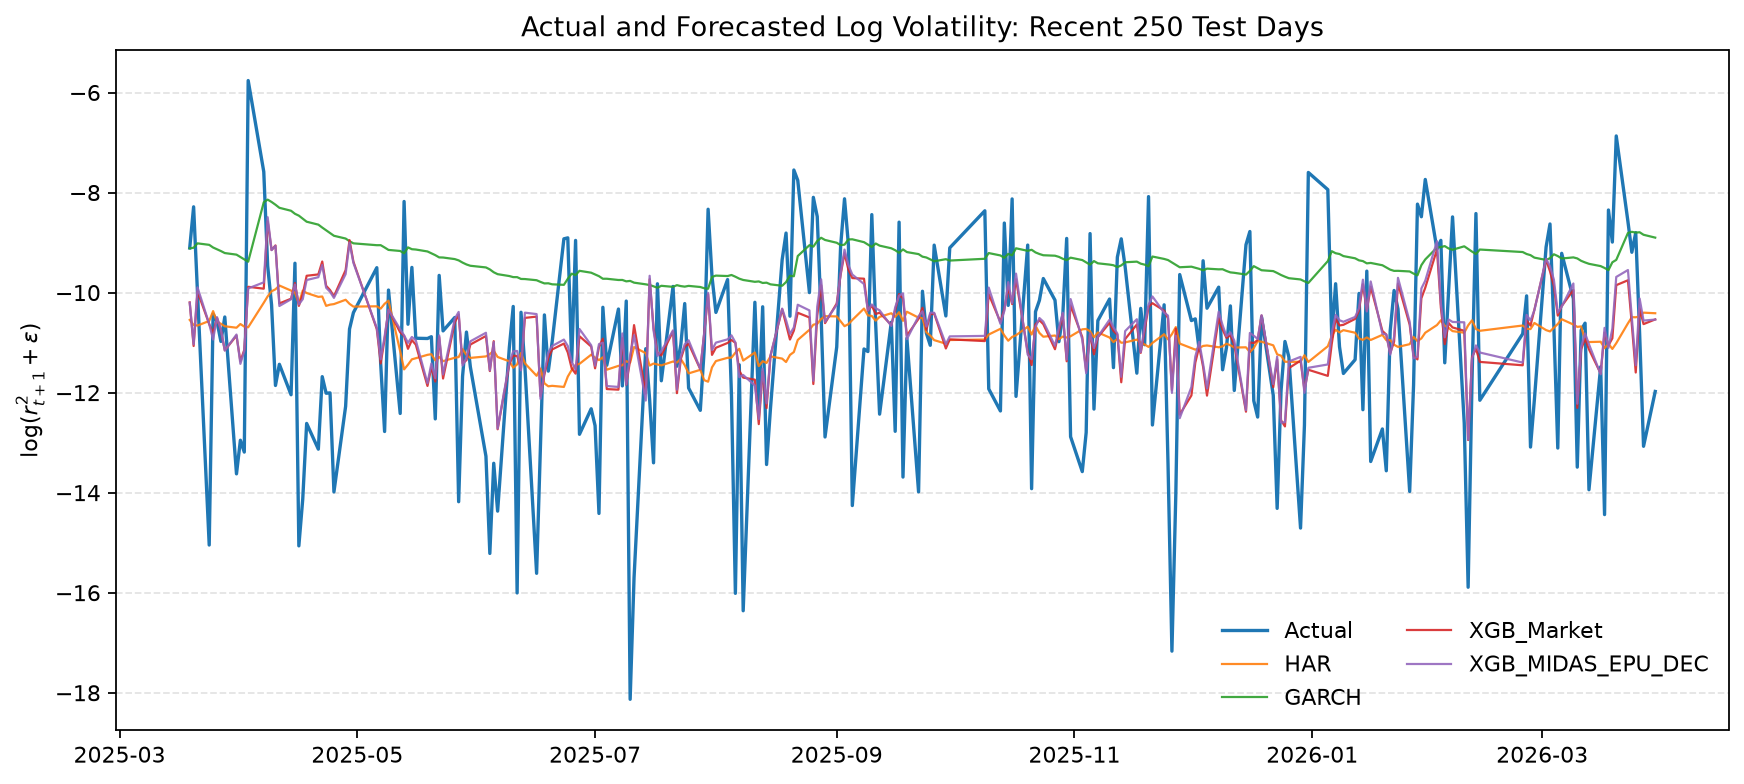
\includegraphics[width=\linewidth]{../../results/revised/sse50/fig_prediction_series_recent.png}\par{\small Recent predictions}\end{minipage}\hfill
\begin{minipage}{.48\textwidth}\centering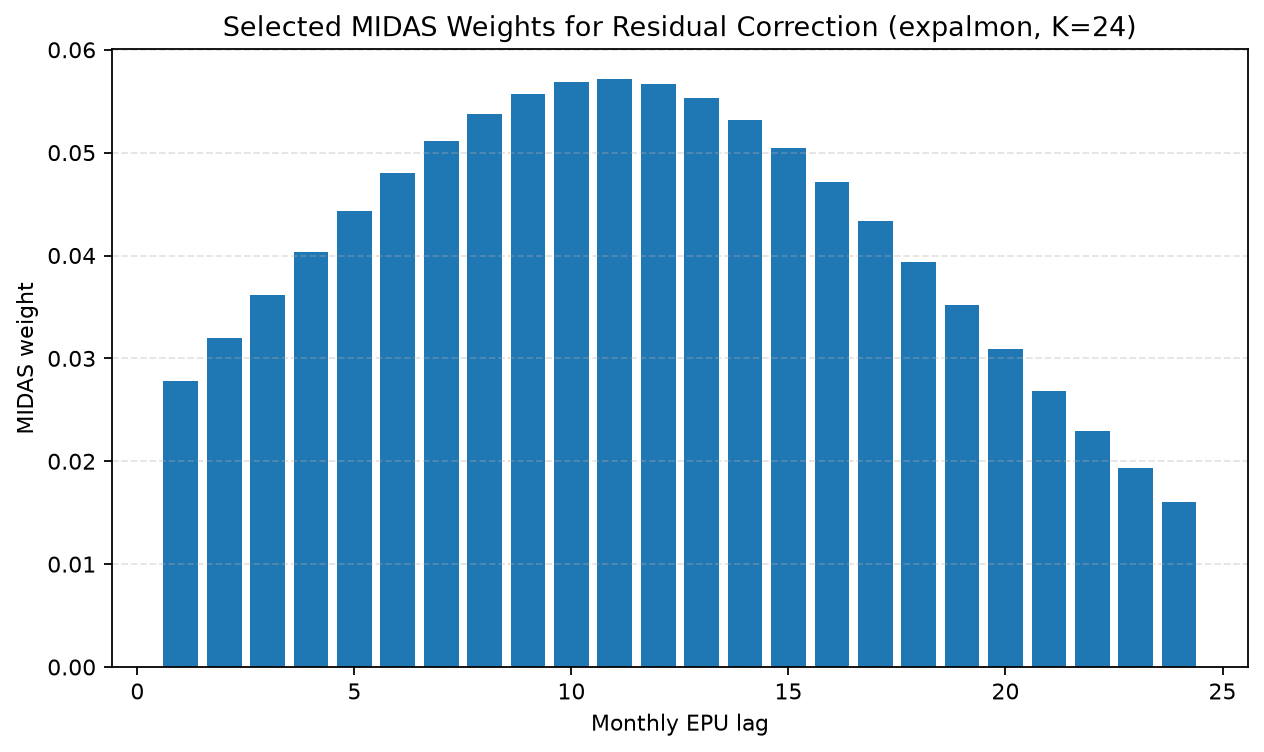
\includegraphics[width=\linewidth]{../../results/revised/sse50/fig_midas_weights.png}\par{\small Validation-selected weights}\end{minipage}
\caption{Revised SSE50 results after the confirmed holiday correction.}
\label{fig:sse50_robustness_panel}
\end{figure}
\begin{figure}[htbp]\centering
\begin{minipage}{.48\textwidth}\centering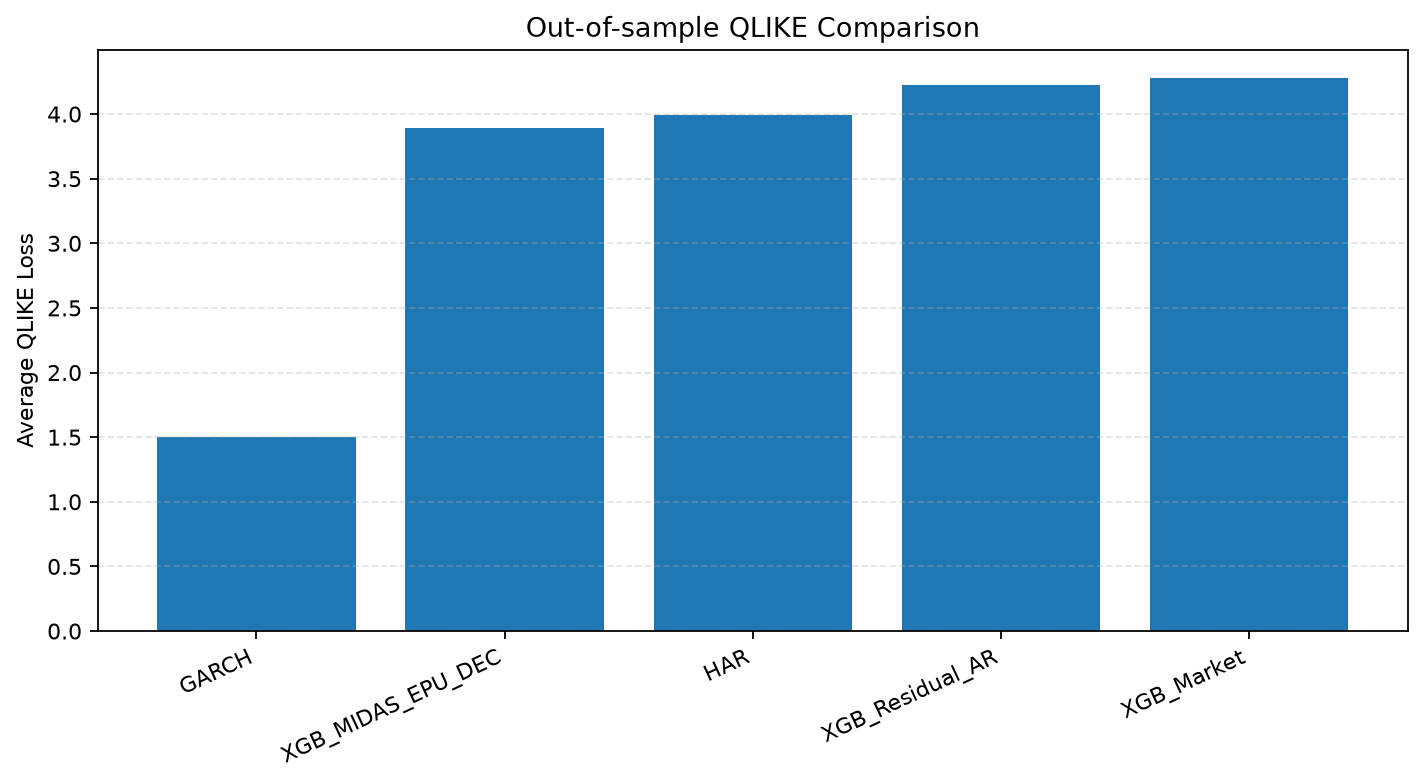
\includegraphics[width=\linewidth]{../../results/revised/nasdaq/fig_metrics_bar.png}\par{\small QLIKE}\end{minipage}\hfill
\begin{minipage}{.48\textwidth}\centering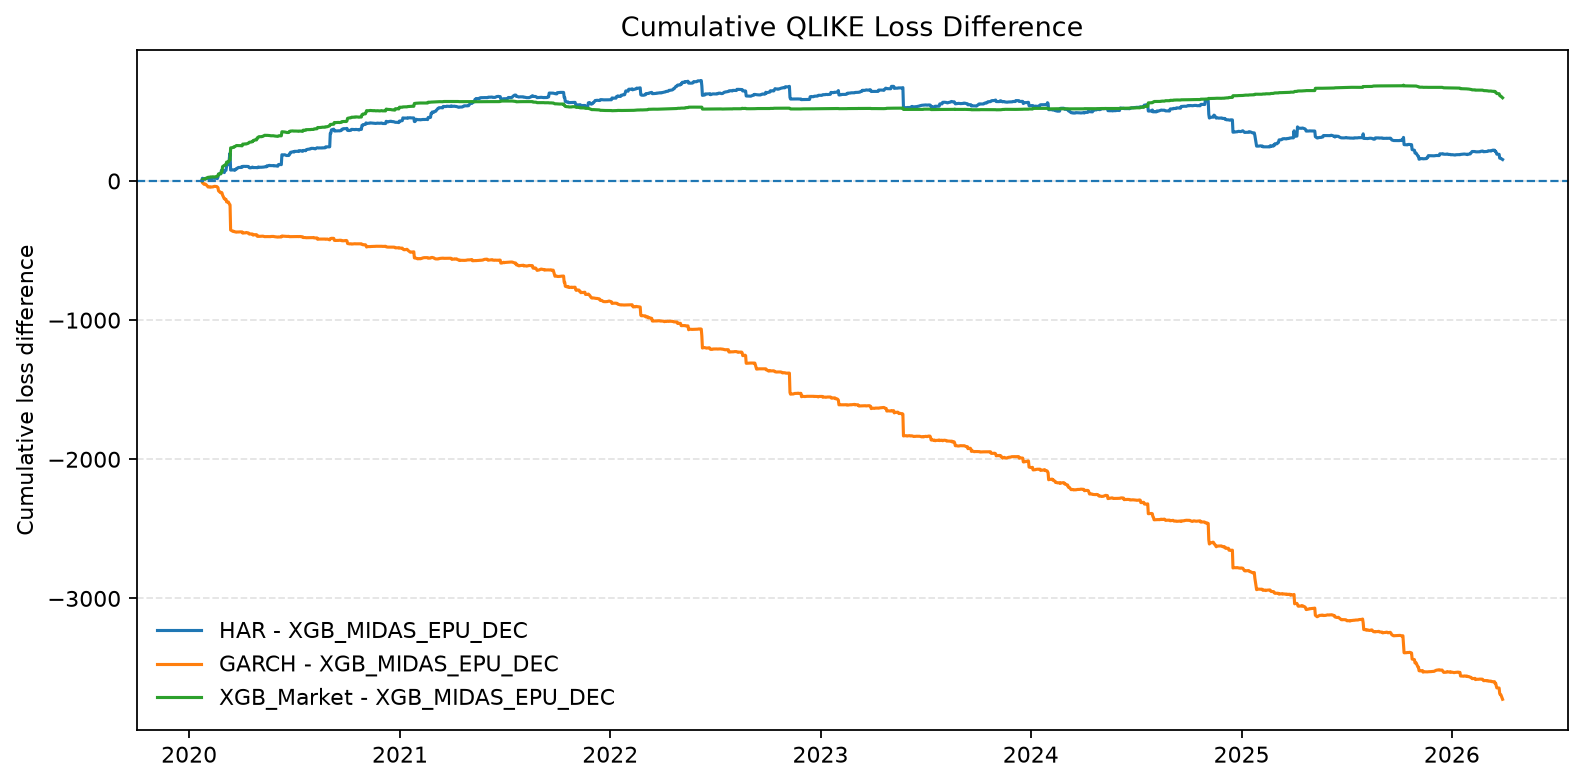
\includegraphics[width=\linewidth]{../../results/revised/nasdaq/fig_cumulative_qlike_diff.png}\par{\small Cumulative QLIKE differences}\end{minipage}\par\medskip
\begin{minipage}{.48\textwidth}\centering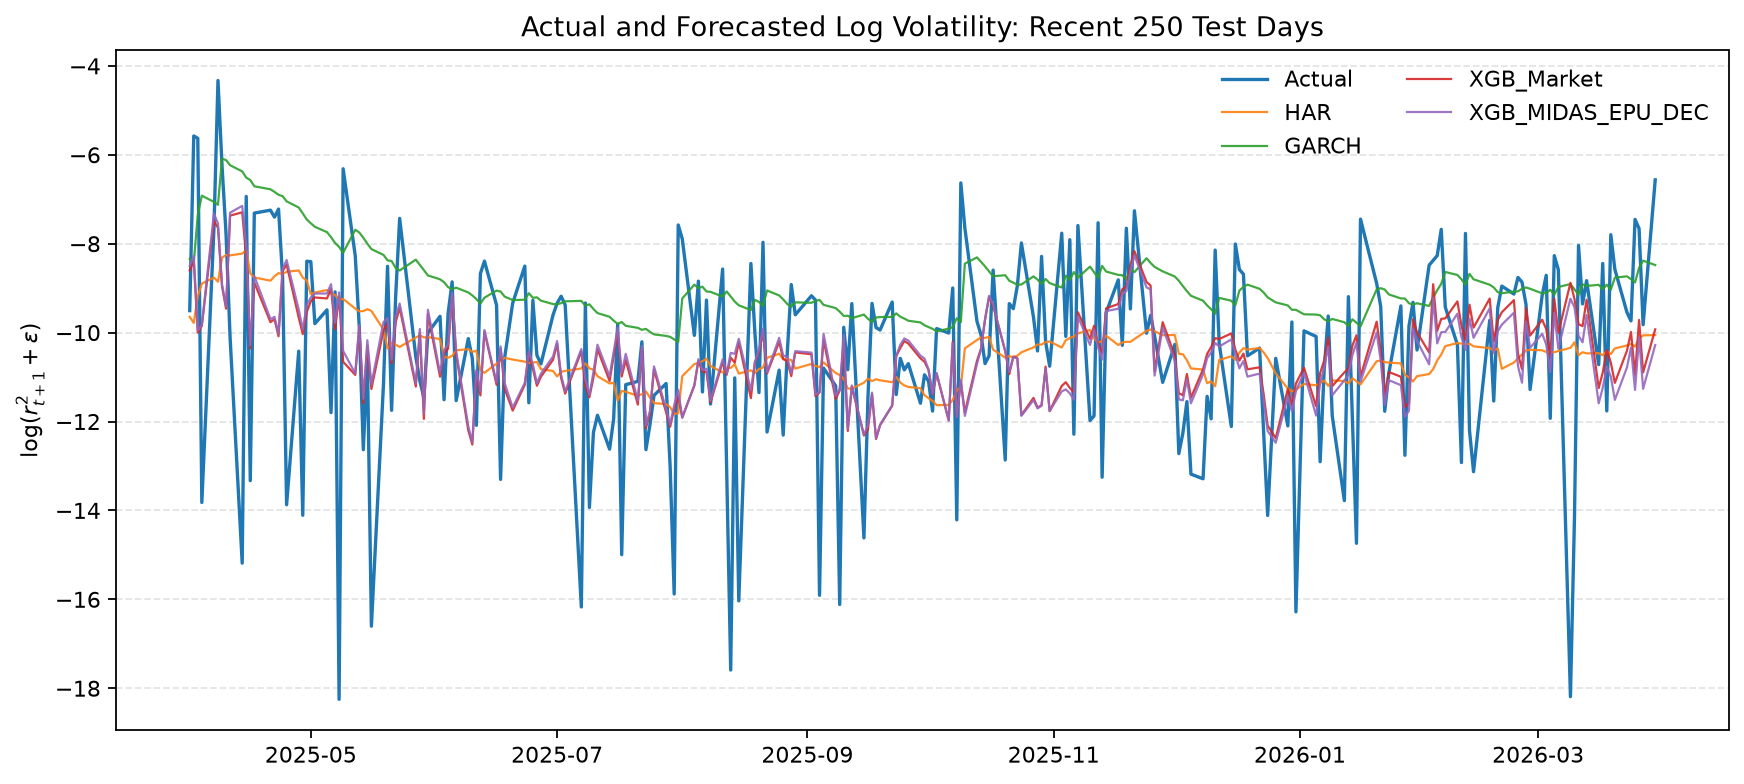
\includegraphics[width=\linewidth]{../../results/revised/nasdaq/fig_prediction_series_recent.png}\par{\small Recent predictions}\end{minipage}\hfill
\begin{minipage}{.48\textwidth}\centering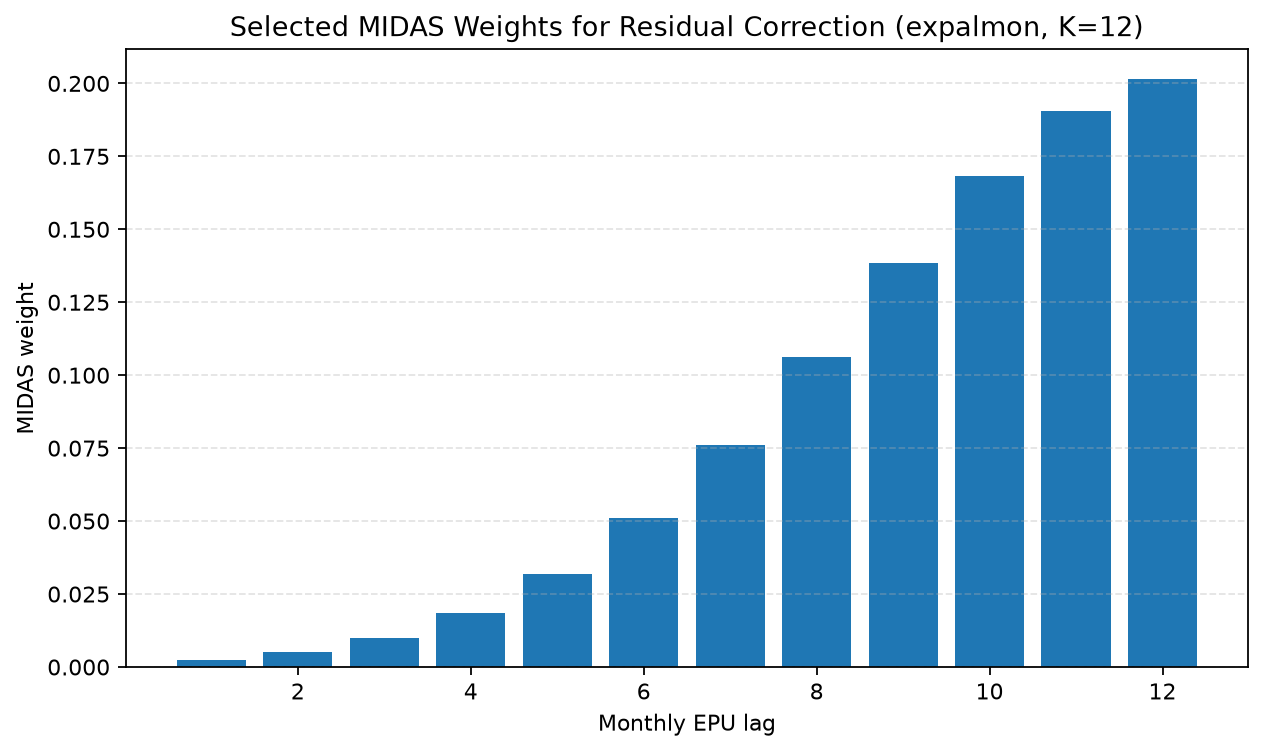
\includegraphics[width=\linewidth]{../../results/revised/nasdaq/fig_midas_weights.png}\par{\small Validation-selected weights}\end{minipage}
\caption{Revised Nasdaq results with the validation-selected Almon specification.}
\label{fig:nas_robustness_panel}
\end{figure}

\subsection{Ablation and scope of evidence}
Mean QLIKE advantages of DEC relative to XGB-AR are 1.168972, 1.025163, and 0.329494 for CSI300, SSE50, and Nasdaq. Holm-adjusted normal-reference $p$-values across the 18 comparisons are approximately $6.61\times10^{-12}$, $4.65\times10^{-7}$, and 0.0215. These are exploratory indications under the retrospective and selection constraints, not conclusive evidence of a population-wide advantage. DEC has higher MSE than XGB-AR in all three markets; the adjusted diagnostics do not support MSE improvement.

A useful next evaluation would lock the entire pipeline in advance, retain genuine release-time EPU vintages, and use a new time holdout. That design would test whether the observed loss-dependent pattern persists beyond the already examined samples.
\clearpage

\clearpage\section{Conclusion}
This study revises a two-stage stock-index volatility-proxy forecasting exercise by separating numerical reproduction, data correction, and predictive evaluation. A sampling-compatible XGBoost build reproduces all 6888 archived first-stage predictions. The original DEC environment cannot be uniquely reconstructed, so the current method uses an explicitly defined profiled objective, analytic gradients, deterministic bounded multistart search, and stationarity checks. The confirmed SSE50 holiday record is removed before feature and target construction, and XGB-AR supplies a residual-only ablation.

The substantive conclusion is conditional on the loss function. Relative to XGB-Market and XGB-AR, revised DEC reduces QLIKE but increases log-MSE in all three markets. MAE improves in the two Chinese markets but worsens in Nasdaq. GARCH remains the best QLIKE benchmark in these comparisons. Improved numerical optimization is valuable for method correctness even when a test metric deteriorates: Nasdaq's validation-selected switch from Beta to exponential Almon improves MSE relative to archived DEC but worsens QLIKE.

Interval evaluation does not support a parallel advantage. On the 1859 common CSI300 dates, the main DEC interval score is 10.1995, worse than HAR's 9.6973, XGB-Market's 9.8534, and XGB-AR's 9.8793. Non-rejection of coverage diagnostics in the main setting does not establish validity, and the 95\%/120-window setting still shows rejection of violation independence and conditional coverage. These are intervals for an observed daily proxy under a specific residual-calibration rule, not confidence intervals for latent variance.

The methodological value is the explicit separation of archived evidence from revised findings, the loss-dependent residual ablation, and the numerical checks. The study does not establish a new general forecasting theorem, an exhaustive advantage over modern alternatives, a global optimizer, or a causal policy mechanism. Weight parameters at their bounds should not be treated as robust economic transmission estimates.

Important limitations remain. The daily proxy is noisy, the log transformation changes the prediction functional, real-time EPU release and revision histories are missing, and the full upstream calendar and data lineage are not independently audited. Historical results were already observed, and the comparison markets are not untouched holdouts. HAC and Holm calculations are therefore exploratory rather than confirmatory. Further work should prioritize a locked design, genuinely available-at-origin inputs, an independent future holdout, and stronger directly implemented benchmarks before making operational forecasting claims.

\clearpage\phantomsection\addcontentsline{toc}{section}{References}
\nocite{*}\bibliographystyle{plainnat}\bibliography{../references}
\clearpage\appendix
\section{Training configuration, platform sampling, and historical controls}
\label{app:training}
The surviving main script and historical discussion records use depth 4 and 300 trees. Changing Python dependency versions alone did not match the archive. Holding inputs and parameters fixed while replacing the platform-dependent column-shuffle behavior allowed XGBoost 2.0.3 CPU histogram training to reproduce all 6888 archived predictions. The compatibility path follows Microsoft STL 17.6 sampling behavior while retaining the original mt19937 engine. It does not search random seeds or optimize test losses to fit historical outputs. Native macOS sampling remains a nonmatching control.

This establishes a numerically equivalent configuration, not unique identification of the original compiler, operating system, installed package version, or complete library stack. The former appendix's depth 3, minimum child weight 5, zero $L_1$ penalty, and early stopping after 50 rounds do not describe the matched experiment. Table~\ref{tab:training_configuration} gives the corrected record.

\begin{table}[htbp]\centering\small
\caption{Configuration numerically matching the archived XGBoost forecasts.}
\label{tab:training_configuration}
\begin{tabularx}{\textwidth}{lX}\toprule Parameter & Value or behavior\\\midrule
\texttt{n\_estimators / learning\_rate} & 300 / 0.05\\
\texttt{max\_depth / min\_child\_weight} & 4 / 3\\
\texttt{subsample / colsample\_bytree} & 0.8 / 0.8\\
\texttt{reg\_alpha / reg\_lambda} & 0.1 / 1.0\\
\texttt{objective / random\_state} & Squared error / 2026\\
Tree construction / maximum bins & CPU histogram / 256\\
Initial intercept & Estimated from training labels at each fit\\
Column sampling & Microsoft STL 17.6-compatible shuffle\\
Early stopping, winsorization, scaling & None in this matched workflow\\
HAR / XGB / GARCH refit interval & 20 retained observations\\
MIDAS refit interval & 60 retained observations\\
MIDAS candidates & 6, 12, 24 months; Beta and exponential Almon\\\bottomrule
\end{tabularx}
\end{table}

Historical train/validation/test counts are 1500/500/1919 for CSI300, 1500/500/1915 for SSE50, and 2000/500/1554 for Nasdaq. The nine market features retain their configured order. Thread counts 1, 2, 4, 8, and the default give identical predictions in the first-validation-block control; the full matching run uses four threads.

\subsection{Full historical reproduction}
Table~\ref{tab:reproduction_difference} compares reconstructed-input forecasts with archived predictions. XGBoost differences cover validation and test predictions; DEC differences cover the test period. In this historical reproduction stage, DEC uses the newly retrained, matching XGBoost predictions, not an archived first-stage prediction cache.

\begin{table}[htbp]\centering
\caption{Maximum absolute log-forecast differences from the archive after sampling compatibility.}
\label{tab:reproduction_difference}
\begin{tabular}{lrrr}\toprule Market & XGB predictions & XGB difference & DEC difference\\\midrule
CSI300 & 2419 & 0 & 0.002670\\
SSE50 & 2415 & 0 & $1.28\times10^{-5}$\\
Nasdaq & 2054 & 0 & 0.003035\\\bottomrule
\end{tabular}
\end{table}

Legacy DEC still fails a uniform absolute tolerance of $10^{-6}$. With baseline forecasts fixed, changing numerical-library combinations or round-tripping equivalent inputs through CSV causes small second-stage differences. These controls demonstrate sensitivity but do not uniquely identify the cause of the historical discrepancy. The legacy specification family and lag length remain unchanged in that forensic comparison. Original plot metadata identifies Matplotlib 3.7.2, which cannot identify the original SciPy or XGBoost versions.

An earlier native-macOS XGBoost 3.4.1 run had maximum cross-market differences of $4.62\times10^{-14}$ for HAR, $7.14\times10^{-5}$ for GARCH, 1.7851 for XGBoost, and 1.5048 for DEC. That run is distinct from the compatible 2.0.3 experiment. The ordinary \path{requirements-reproduction.txt} is not a unique historical lockfile. Installing an official macOS 2.0.3 wheel alone does not supply the compatible column sampling; build instructions, patch provenance, and runtime fingerprints are recorded separately.

\subsection{Separate SSE50 calendar-control experiment}
The earlier calendar control retrained four models with the same compatible build and numerical environment, once on original inputs and once after deleting the confirmed 2018-06-18 holiday before reconstruction. Table~\ref{tab:calendar_sensitivity} evaluates both sets of forecasts on the same 1915 dates and uses the corrected target for both. It retains the legacy single-start DEC method, so it must not be confused with the current five-model stable-solver results.

\begin{table}[htbp]\centering\small
\caption{Historical calendar control on common dates with a unified corrected target.}
\label{tab:calendar_sensitivity}
\begin{tabular}{lrrrr}\toprule
& \multicolumn{2}{c}{MSE} & \multicolumn{2}{c}{QLIKE}\\
Model & Original inputs & Corrected inputs & Original inputs & Corrected inputs\\\midrule
HAR & 4.820334 & 4.820717 & 3.877497 & 3.874467\\
GARCH & 7.521221 & 7.524687 & 1.585780 & 1.585427\\
XGB-Market & 4.902582 & 4.933710 & 4.507373 & 4.756812\\
DEC & 4.931264 & 4.962050 & 3.528922 & 3.672719\\\bottomrule
\end{tabular}
\end{table}

QLIKE ordering in this control remains GARCH, DEC, HAR, then XGBoost, but the values change. The effects include rolling features, training observations, and refit positions, not merely one artificial target. Deleting a single loss observation cannot substitute for reconstructing the pipeline. This control does not resolve all calendar validity, EPU release timing, or numerical-estimation issues.

\section{Verification of the revised DEC method}
\label{app:solver}
Legacy DEC reproduction on historical inputs changes CSI300 MSE by approximately $+0.000094$ and QLIKE by $-0.000362$ relative to the archive. SSE50 and Nasdaq show extremely small decreases in MSE, MAE, and QLIKE. Those are numerical-environment differences and do not reverse the model rankings. The stable-method revision in the main text is a separate experiment, not exact restoration of legacy DEC.

The current revision includes three main-market cases plus an SSE50 historical-input control, totaling 146 specification and test-refit estimations. All selected solutions satisfy the mean-SSE projected-gradient threshold of $10^{-6}$; the largest diagnostic is about $2.09\times10^{-9}$. Independent bounded finite-difference checks for the 108 main-market fits give a maximum projected gradient of about $2.10\times10^{-9}$. The new training SSE is no greater than the corresponding single-start value within a numerical tolerance of $10^{-7}$. This supports first-order numerical stability, not global optimality.

Holding inputs, first-stage forecasts, and estimation rules fixed, comparisons between NumPy 2.5.4/SciPy 1.18.1/statsmodels 0.15.0 and NumPy 1.26.4/SciPy 1.11.4/statsmodels 0.14.2 give maximum revised DEC forecast differences of $8.05\times10^{-8}$, $9.32\times10^{-8}$, and $4.40\times10^{-8}$ for CSI300, SSE50, and Nasdaq. Each is below $10^{-7}$. Repeating from saved inputs within the same environment gives identical predictions. These are the tested stacks, not a claim of invariance across every platform or dependency version.

In the current research revision, DEC, XGB-AR, HAR, and GARCH are re-estimated. The first stage reuses a previously verified local XGBoost cache after checking dates, sample flags, targets, and SHA256. The public current entry point can retrain XGBoost from authorized raw inputs; cache reuse is a documented acceleration option. It is not described as a new full first-stage training run.

Current and historical comparisons, six-candidate searches, optimizer diagnostics, dependency records, and all 30 common-date interval settings are supplied under \path{results/revised/}. Per-period private inputs, predictions, models, and local logs are excluded from the distribution. The synthetic example uses invented data to exercise the implementation and does not reproduce the paper's empirical results.

\section{Verification scope and source attribution}
The public research archive preserves the core model definitions and historical outputs. Current text uses stable estimation, residual ablation, and common-date evaluation; historical figures and tables remain in their original result directories. Arithmetic checking, input reconstruction, candidate retraining, and second-stage checks with fixed baseline forecasts are recorded separately. None alone establishes that all original inputs were genuinely available at their recorded forecast origins.

Detailed public checks are in \path{results/verification/}, with calculation procedures including \path{scripts/audit_results.py}. The original long literature excerpts were replaced by brief reading notes: \citet{BakerBloomDavis2016} develops news-based EPU measurement, and \citet{ChenGuestrin2016} describes the XGBoost system. The present rolling absolute-residual intervals do not implement EnbPI \citep{XuXie2021} and cannot directly inherit its theoretical guarantees. Scholarly names and bibliographic institutions are retained for correct attribution; they are not identifying affiliations of this project's author.

\end{document}
